\documentclass[11pt,letterpaper]{article}
\input{headings}
\newcommand \recipeName {Almoronia}
\newcommand \fileName {Almoronia}
\chead{\recipeName}

\begin{document}
\input{title}

Almoronia is a traditional chicken-and-eggplant recipe that was brought to Morocco by the Jewish communities expelled from al-Andaluz. I started with the recipe by Tess Mallos that I found in {\it The food of Morocco: a journey for food lovers} and tried to bring it to our times. Instead of deep frying the eggplant in oil, I use the method of salting, pat drying, grilling and let them finish cooking steaming in a closed container. For the chicken, I use skinless, but bone-in, chicken thighs instead of the whole chicken in the original recipe. Also I replaced the boiling of the chicken with a gentle braising. To ensure the most flavourful and moist meat I borrow a method from the America's Test Kitchen and slow braise the thighs for three hours at very low temperature. This time can be cut in half at a higher temperature with similar results.

\begin{description}

\item[Ingredients:]\ \\
	\begin{itemize}
	\item 1.25 kg (2 3/4 pounds) of bone-in skinless chicken thighs 
	\item 1 teaspoon of freshly ground black pepper
	\item 1 stick cinnamon
	\item 1/4 teaspoon of saffron strands
	\item salt
	\item 750 grams (1 3/4 pounds) eggplants 
	\item canola oil
	\item 2 large onions, peeled and sliced into half moons
	\item 3 tablespoons olive oil
	\item 1 clove of garlic, peeled 
	\item 1 teaspoon of honey
	\end{itemize}

\item[Procedure:]\ \\
	\begin{enumerate}
	\item {\bf Braise the chicken thighs}
	\begin{itemize}
	\item Pre-heat oven to 200 F.
	\item Dissolve the saffron strands into 1/4 cup of water.
	\item Sprinkle the chicken thighs with salt and 1/2 teaspoon of ground black pepper.
	\item Place in an oven-safe dish with a tight cover --- or use a dish without cover and cover tightly with aluminum foil.
	\item Break the cinnamon stick into two pieces and put far apart in the dish. 
	\item Spread the saffron water all over the chicken pieces.
	\item Cover the dish and put in the oven.
	\item Braise for about three hours. The chicken is done when the temperature close to the bone in the thickest pieces reaches 195 F when tested with an instant-reading thermometer.
	\item Alternatively, braise in a 325 F oven for about 80 minutes until the internal temperature reaches 195 F.
	\item Remove from the oven and keep it warm until you are ready to assemble the dish. 
	\end{itemize}
	\item {\bf Grill the Eggplants}
	\begin{itemize}
	\item Cut the ends of the eggplants and, using a vegetable peeler, peel longwise stripes from the eggplants, leaving some strips of the skin.
	\item Cut eggplants into 1 cm (slightly thiner than 1/2 inch) thick slices.
	\item Sprinkle each slice on both sides with salt.
	\item Put the eggplants in a colander and let seat for at least 30 minutes and up to 90 minutes.
	\item Heat up your gas grill to moderate heat level.
	\item Using paper towels, pat the eggplant slices dry.
	\item In a shallow dinner plate put a thick film of canola oil.
	\item Quickly coat both sides of each eggplant slice with the canola oil and place on another dish. Adding more oil as it is absorbed by the eggplant slices.
	\item Clean the grill throughly with a steel brush.
	\item Either spray the grill a few times with cooking spray or put cooking oil in a small dish and using folded paper towels and tongues coat the grill with oil.
	\item Grill both sides of the eggplant slices until they are lightly brown and the eggplant slices are cooked but neither dried up nor mushy. They will continue cooking after removed from the grill.
	\item Transfer the eggplant slices from the grill into a tupperware container with a tight-fitting lead and cover immediately with the lead.
	\item Let the eggplant slices steam on their own heat for at least 20 minutes.
	\end{itemize}
	\item {\bf Brown the onions}
	\begin{itemize}
	\item Heat the olive oil in a heavy pan over moderate heat and add the onions.
	\item Cook for about 30 minutes, stirring regularly until the onions are very tender and reach a pale golden colour.
	\item Stir the honey into the onions and continue cooking while stirring until they reach a deep golden colour. 
	\item Crush the garlic into a paste and add to the cooked onions. Stir for about 30 seconds.
	\item Add the remaining 1/2 teaspoon of black pepper to the onions.
	\item Pour about 2 cups of the juice that accumulated into the chicken onto the onions.
	\item Cook for a further 10 minutes over gentle heat.
	\end{itemize}
	\item {\bf Assemble the Almoronia}
	\begin{itemize}
	\item Preheat oven to 300 F
	\item Lay the cooked eggplant on the bottom of an ovenproof dish.
	\item Remove the bones and any blood vessels from the chicken thighs and break the meat into large pieces with your fingers.
	\item Spread the chicken meat over the eggplant slices.
	\item Pour the onion sauce over the chicken.
	\item Place in the oven and cook for 30 minutes.
	\end{itemize}
	\end{enumerate}
\end{description}
\begin{table}
\begin{tabular}{cccc}
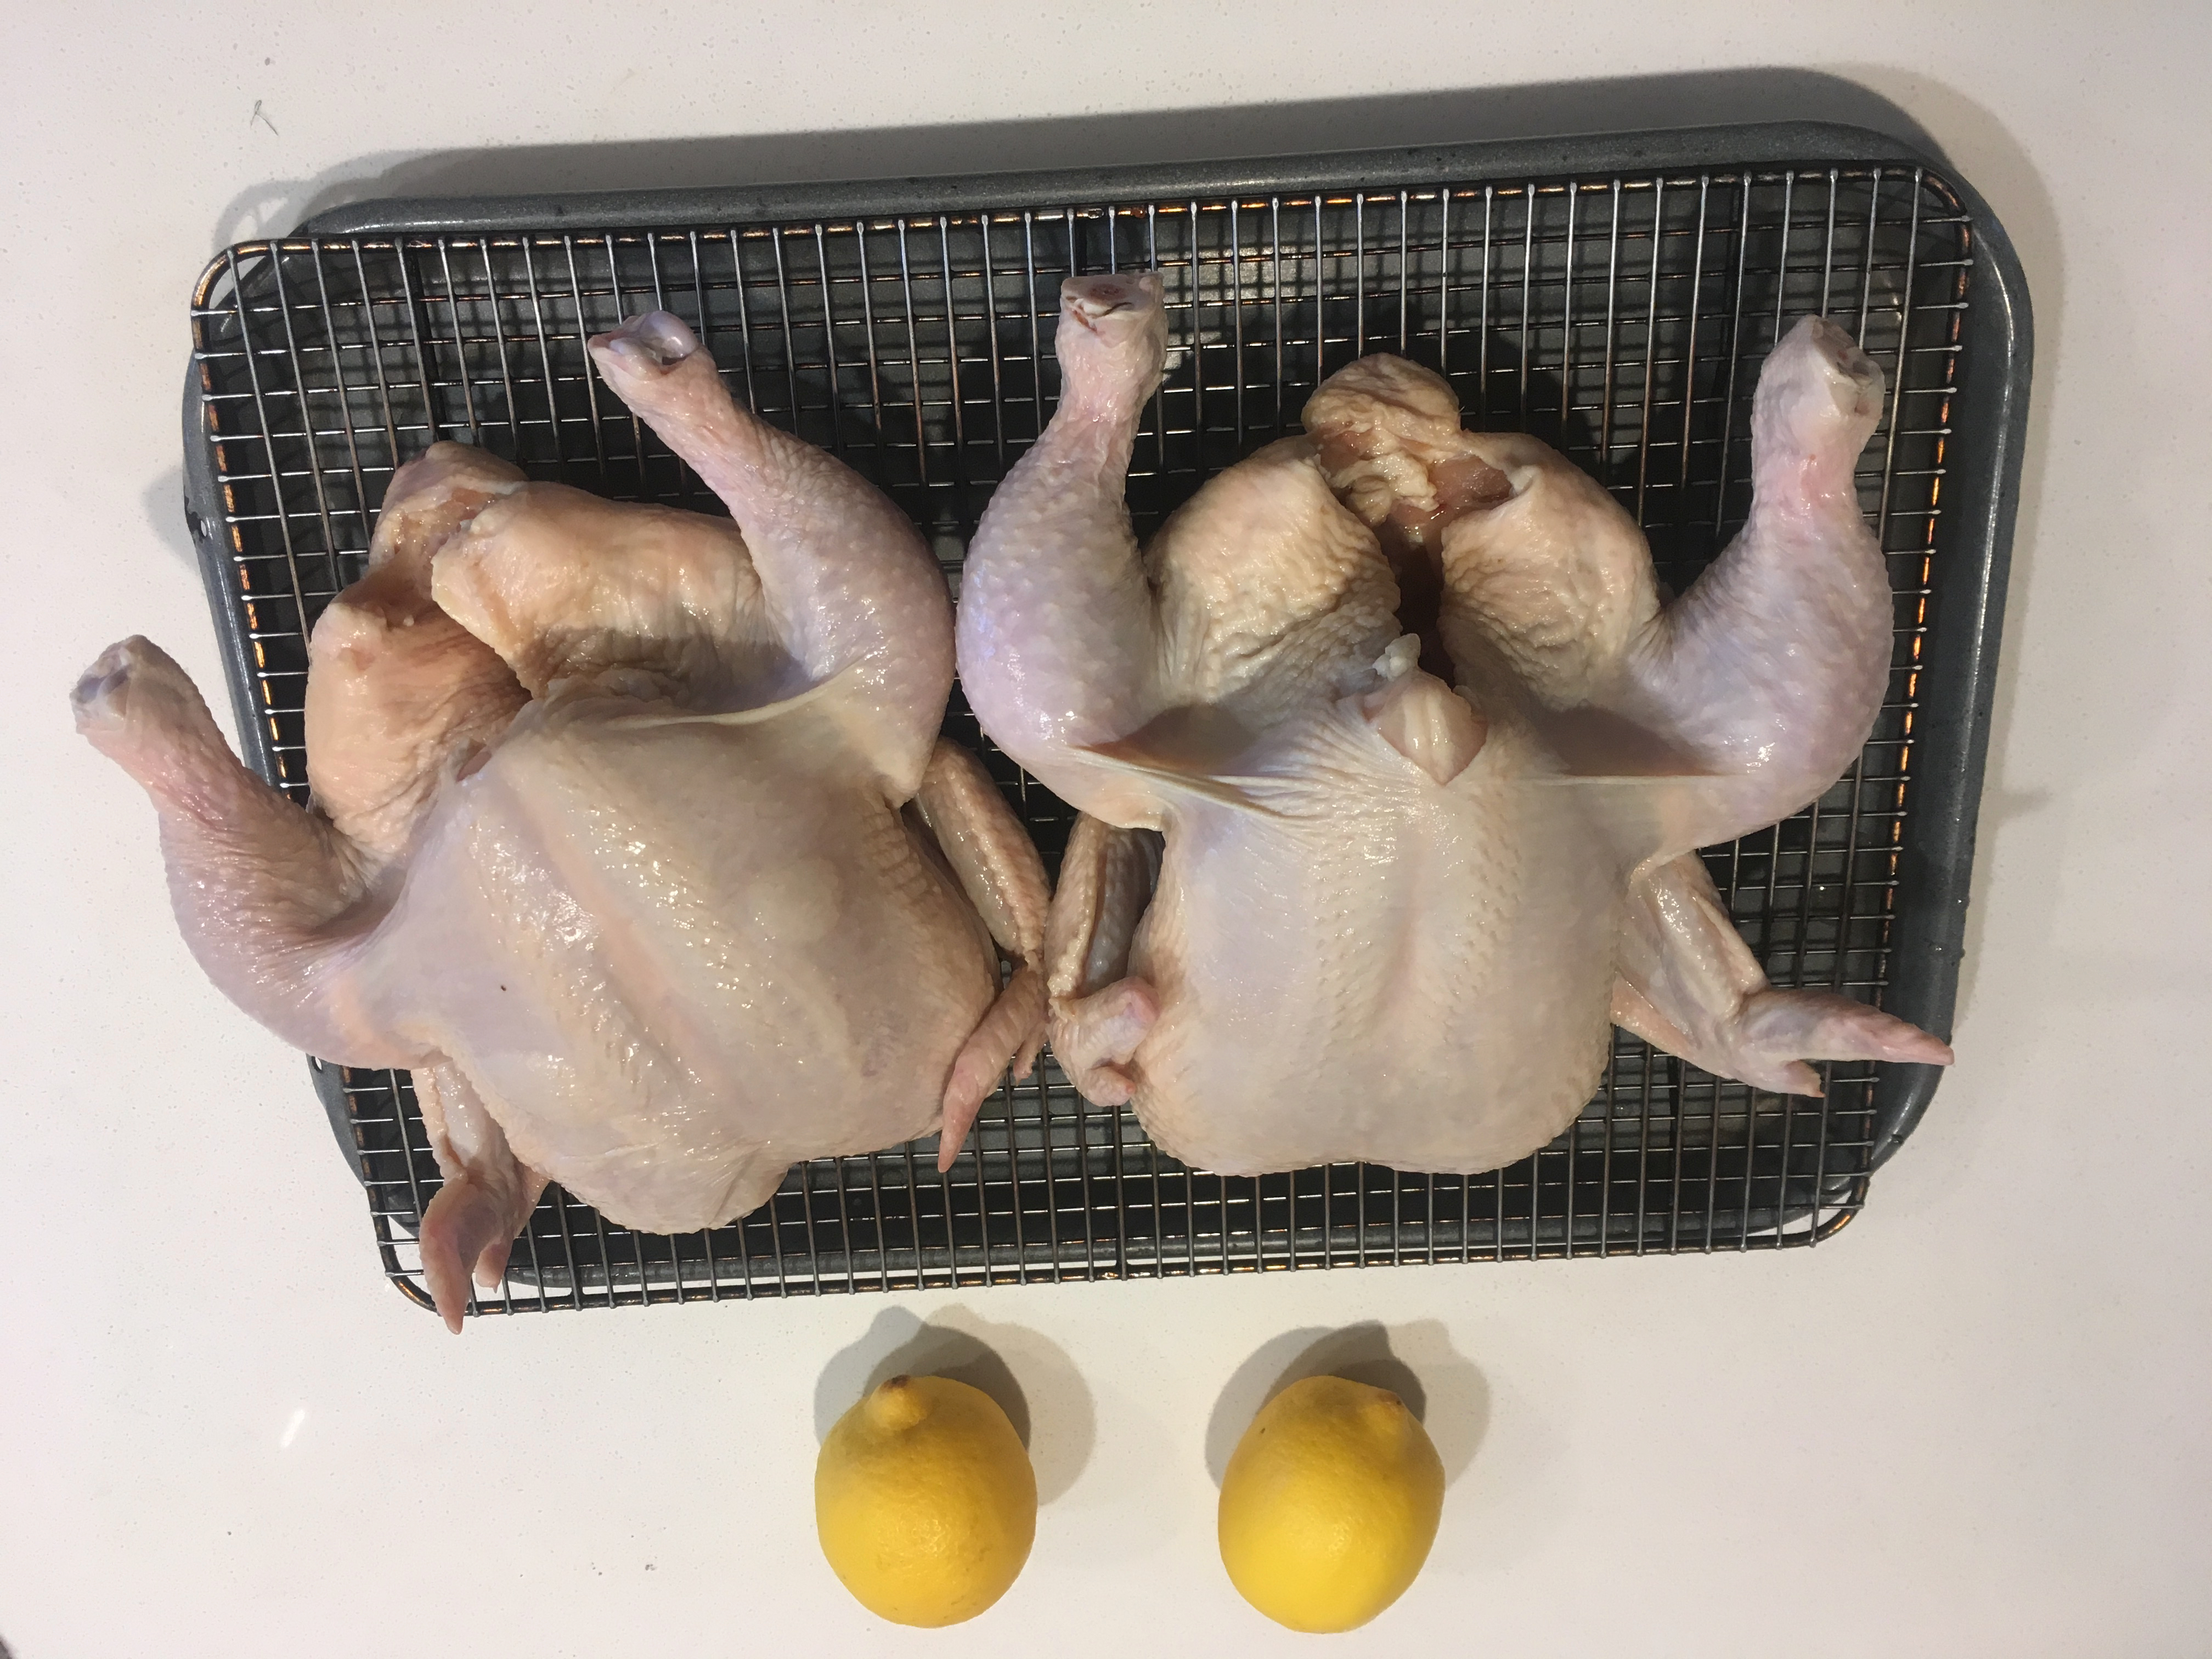
\includegraphics[width=0.25\textwidth]{\imageDir/\fileName/IMG_3197.jpg} &
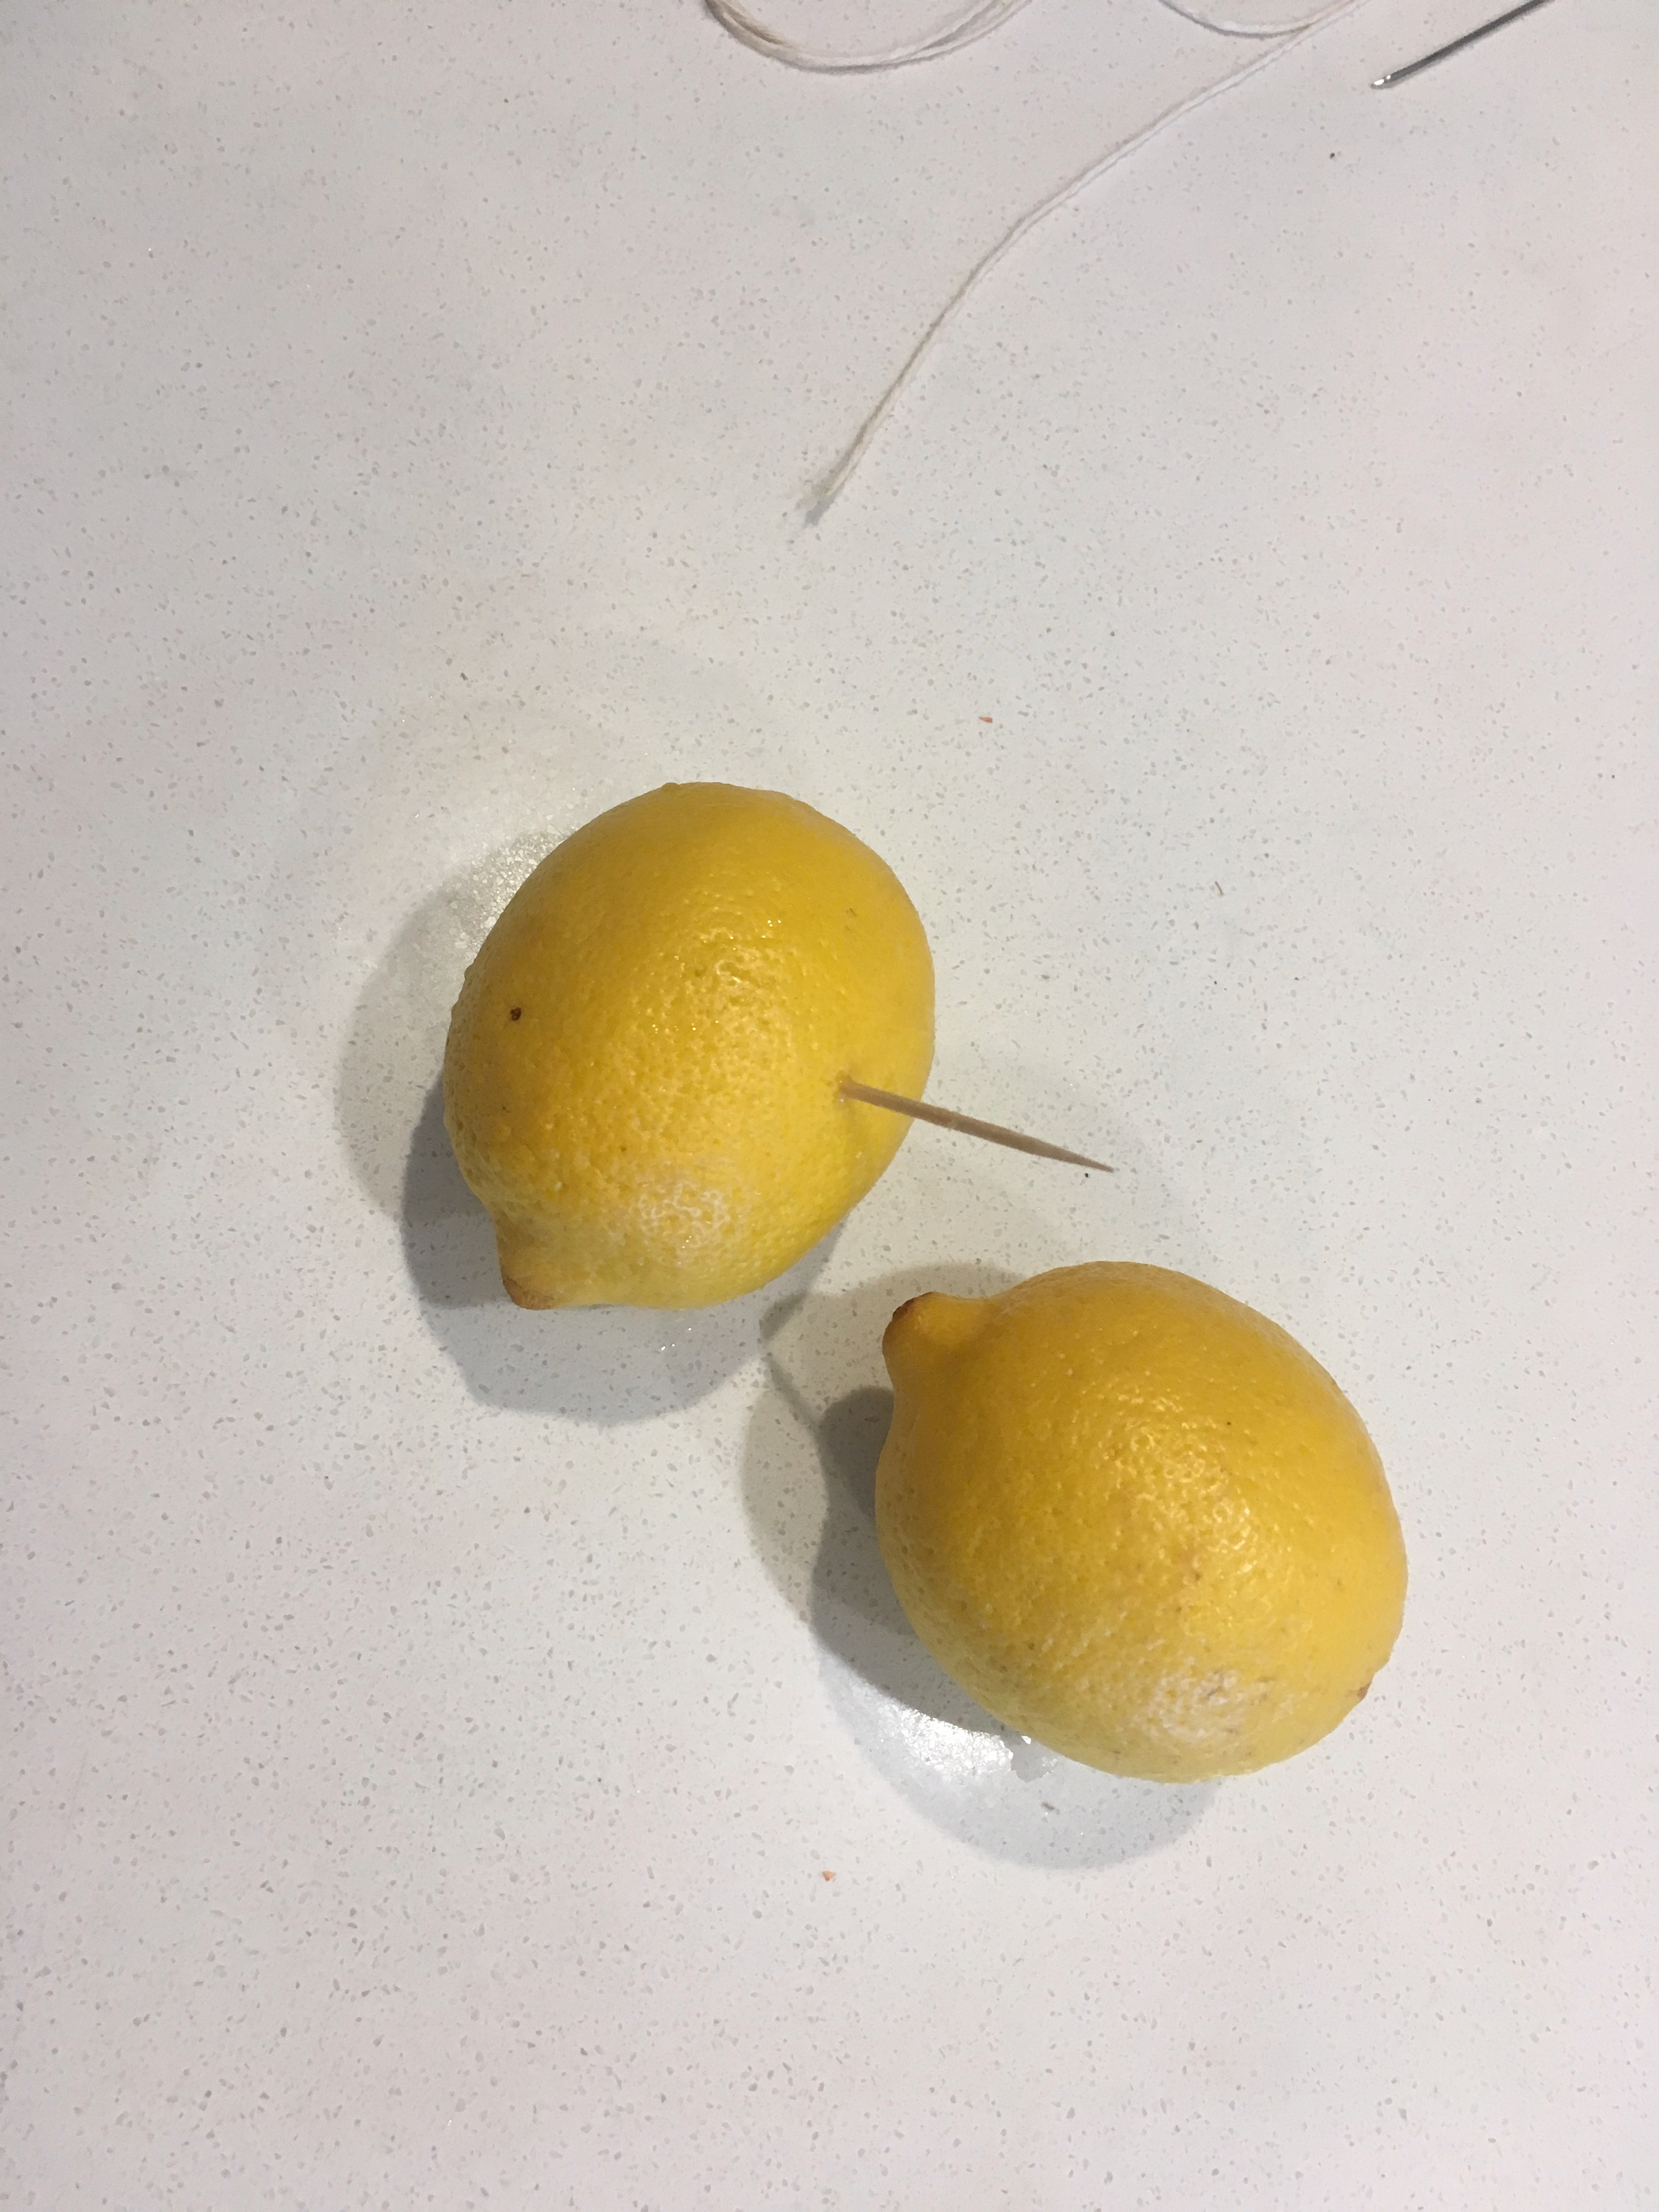
\includegraphics[width=0.25\textwidth]{\imageDir/\fileName/IMG_3212.jpg} &
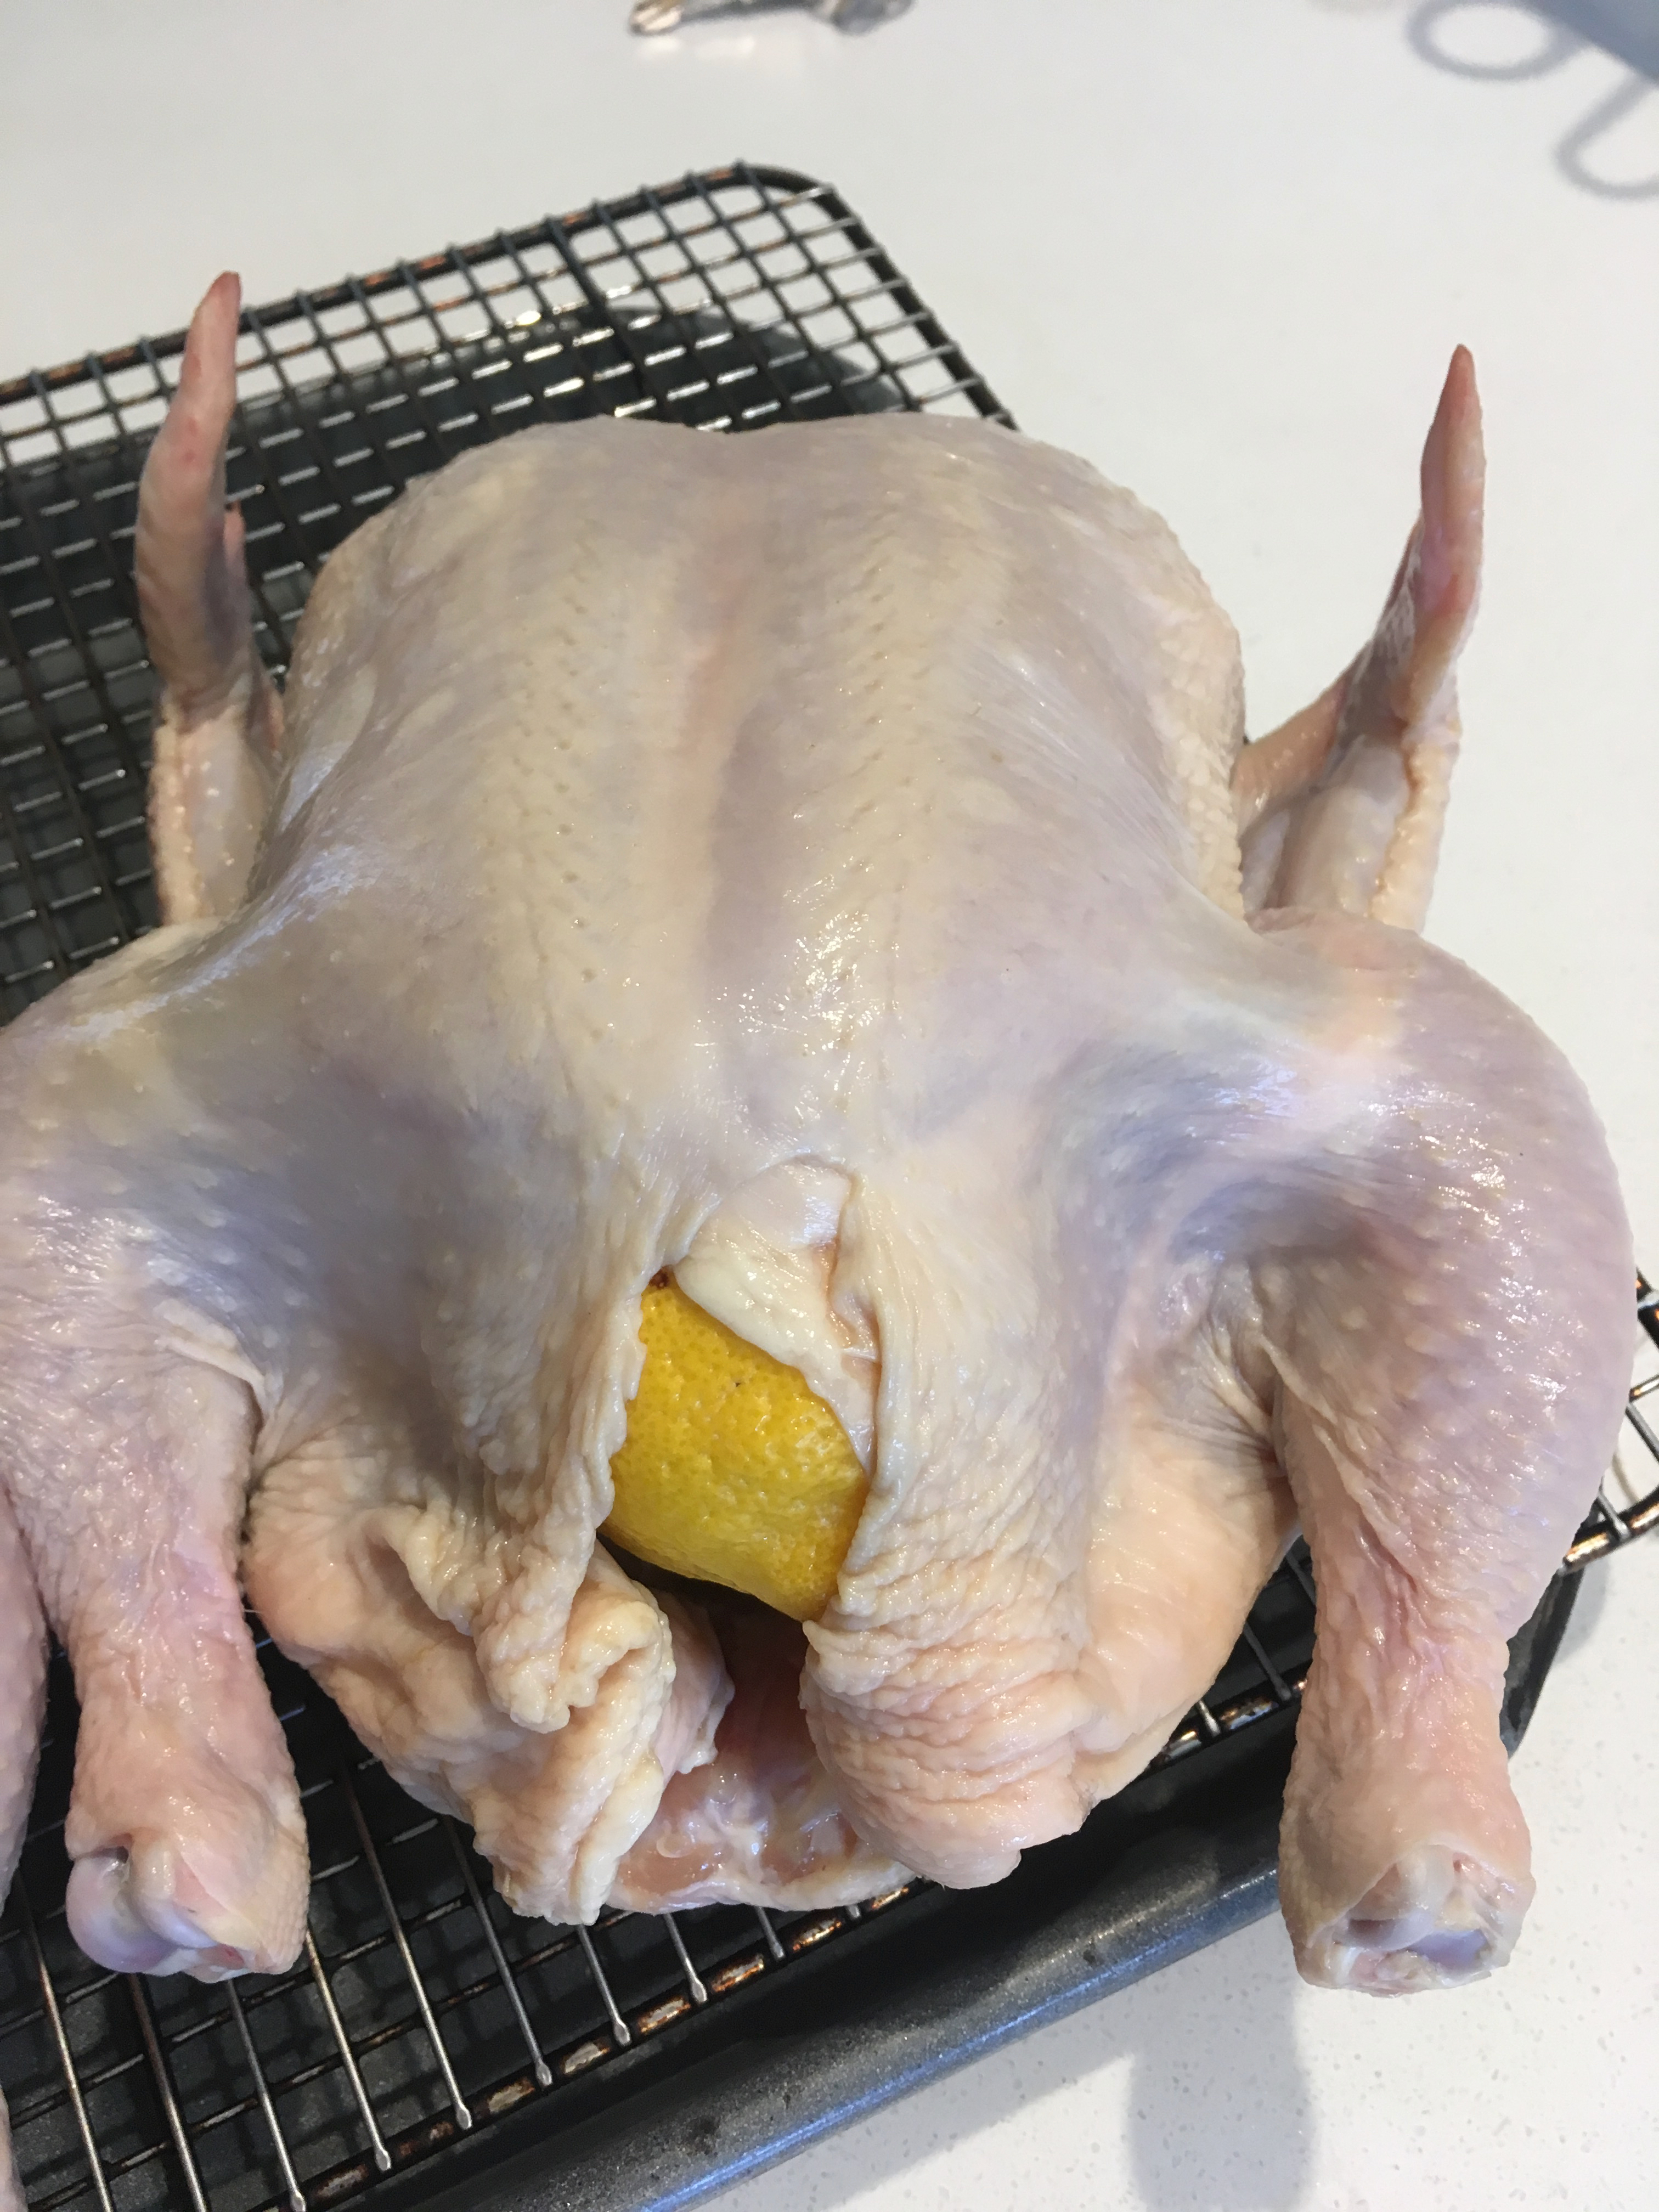
\includegraphics[width=0.25\textwidth]{\imageDir/\fileName/IMG_3213.jpg} \\
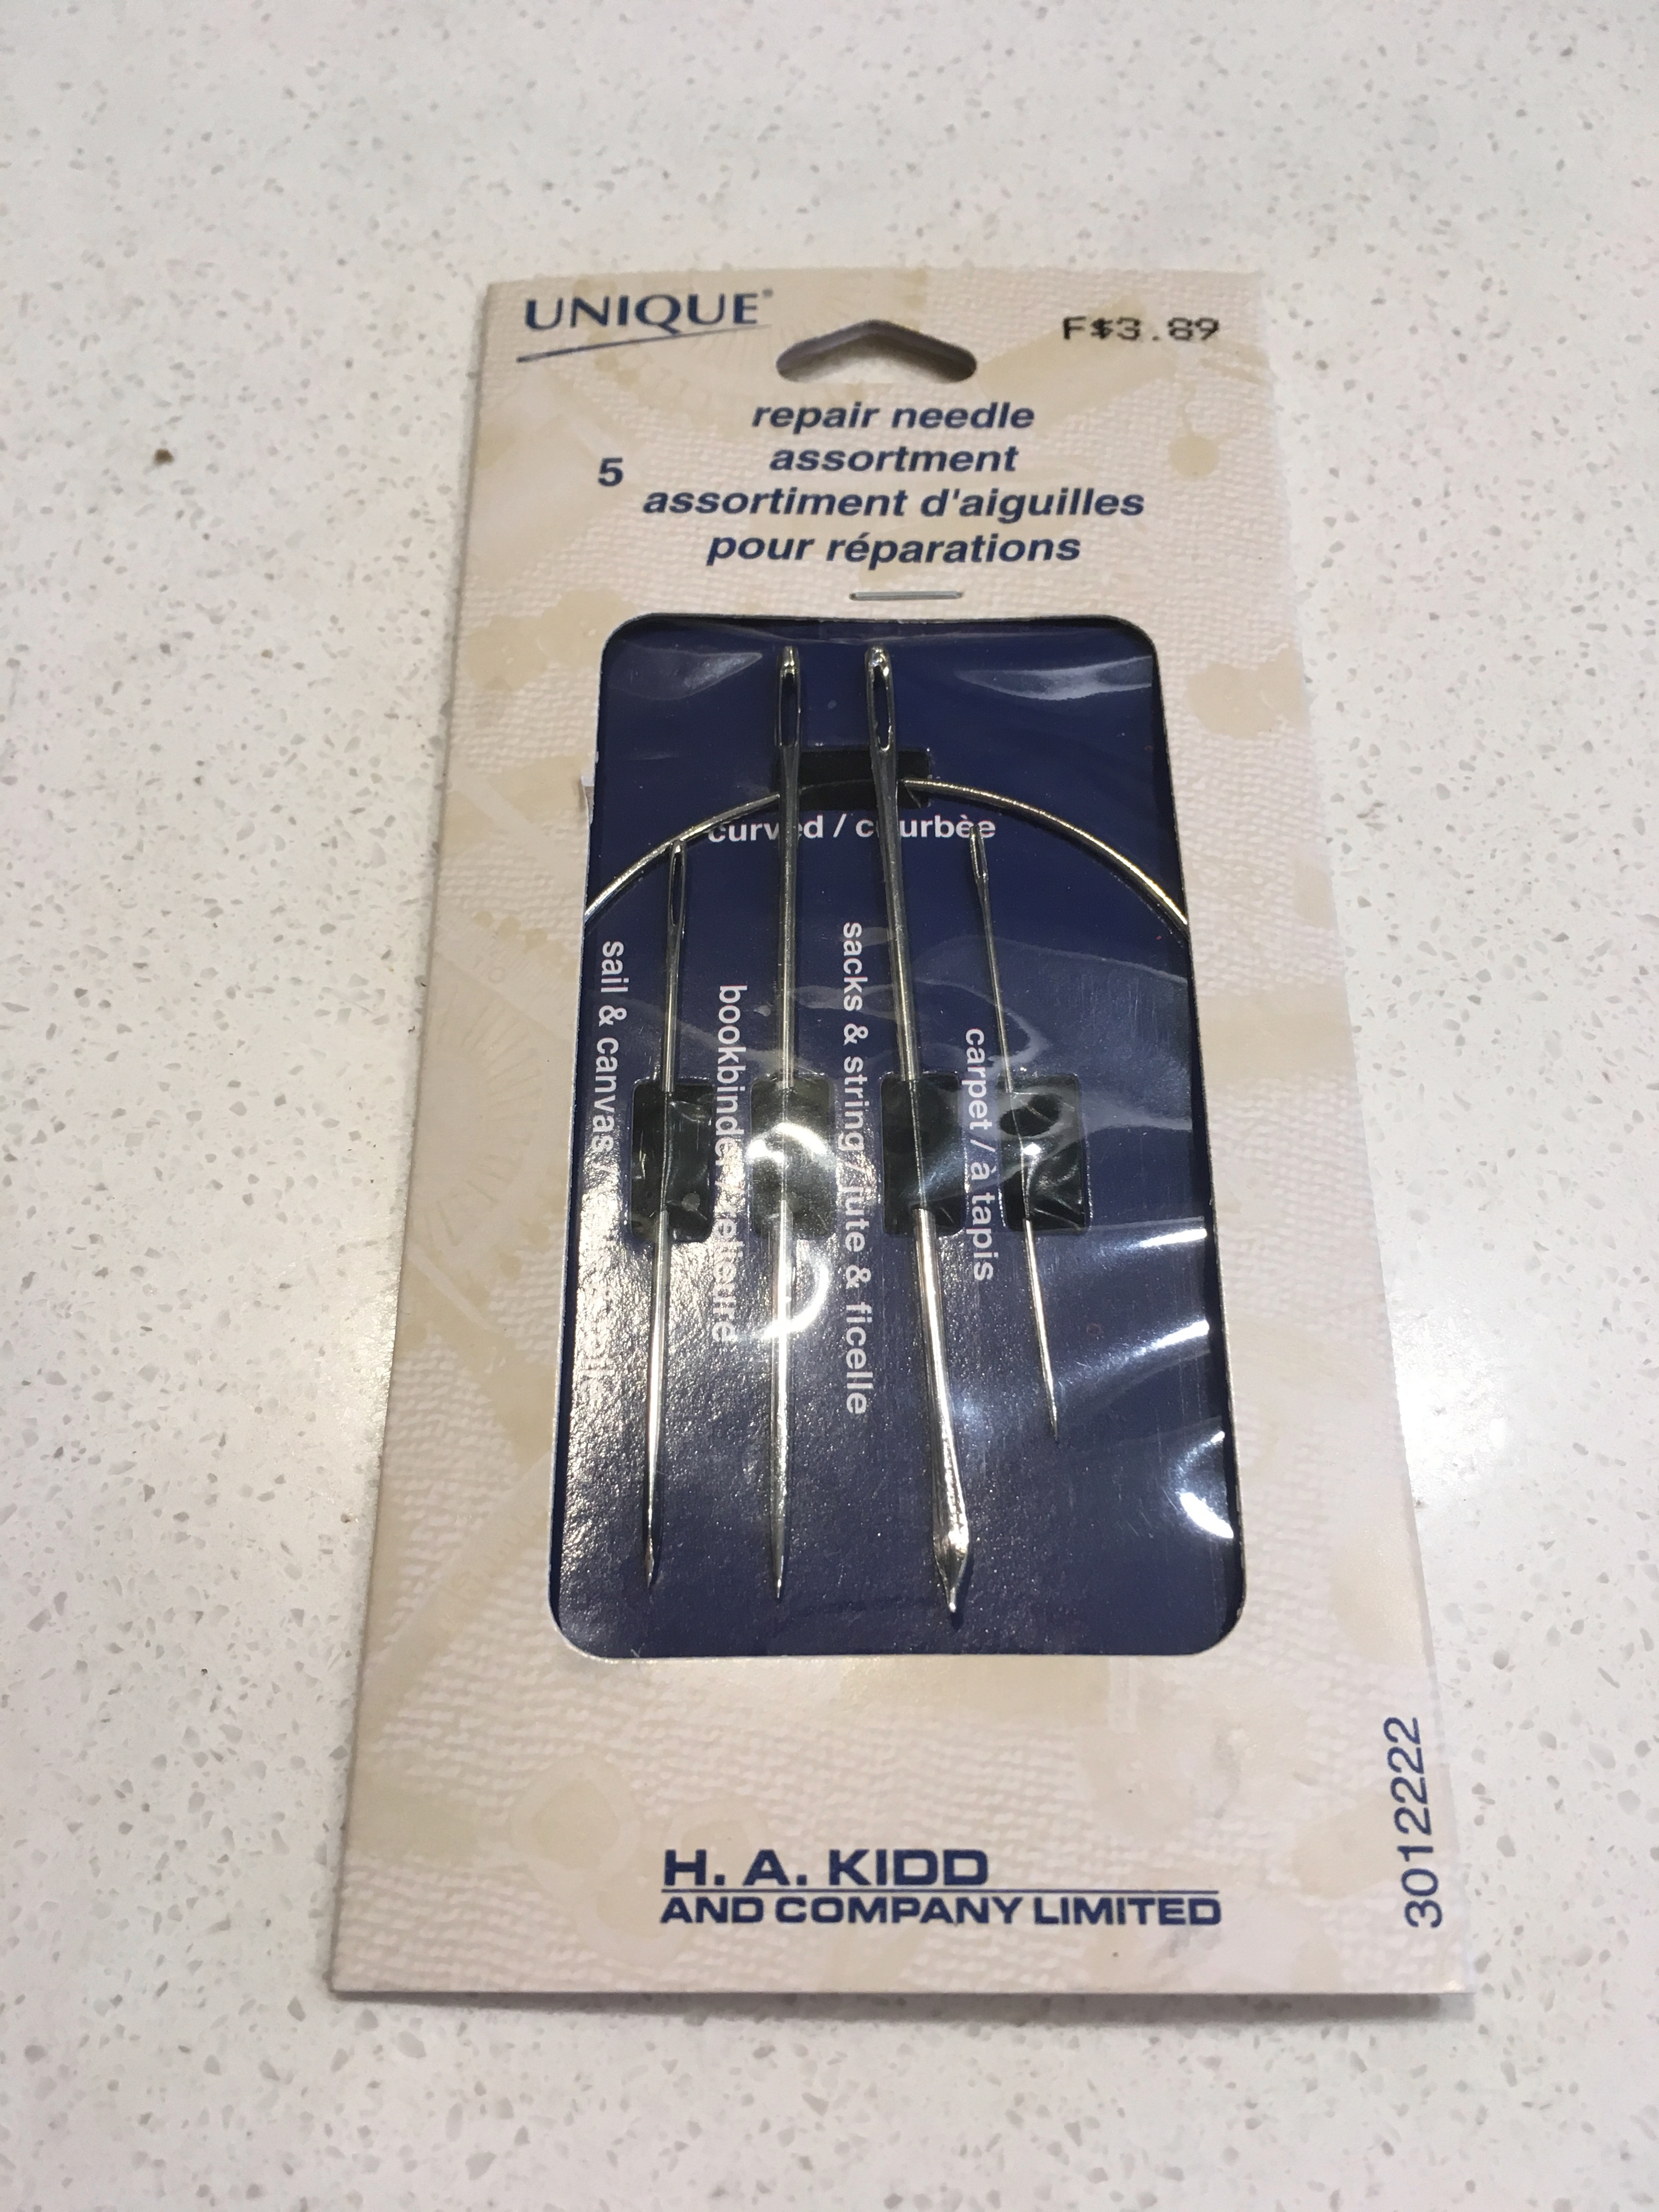
\includegraphics[width=0.25\textwidth]{\imageDir/\fileName/IMG_3206.jpg} &
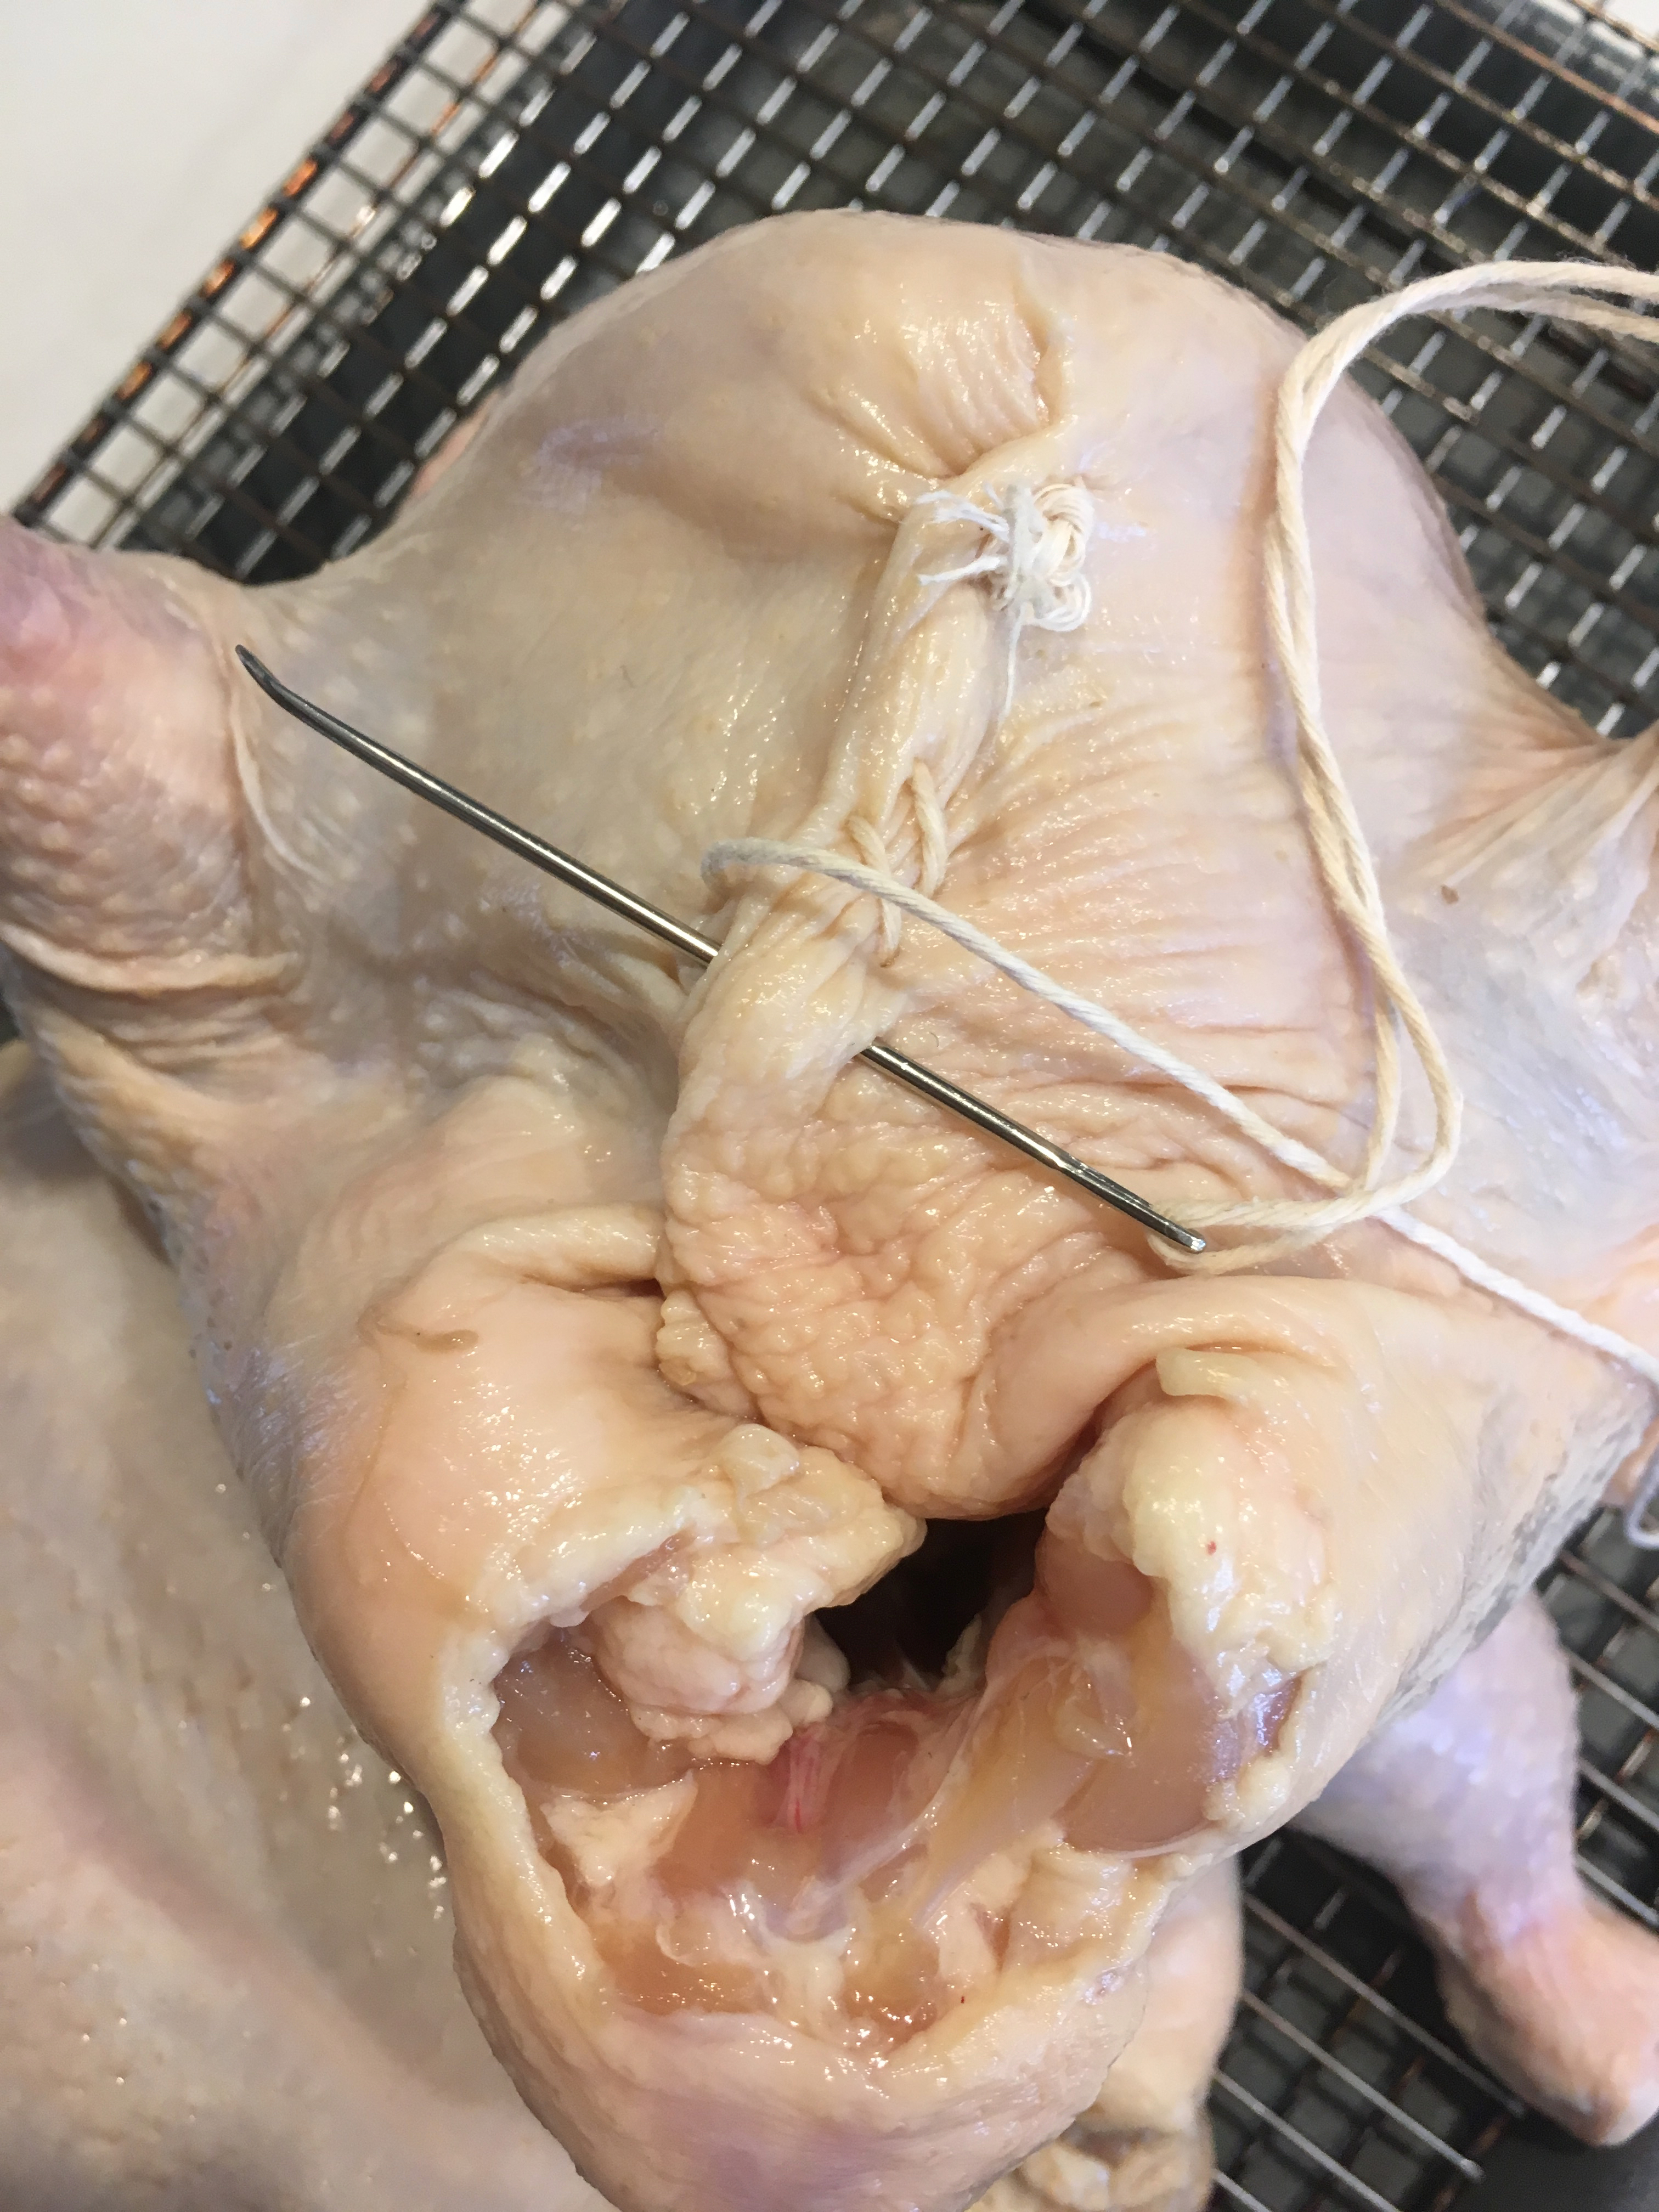
\includegraphics[width=0.25\textwidth]{\imageDir/\fileName/IMG_3214.jpg} &
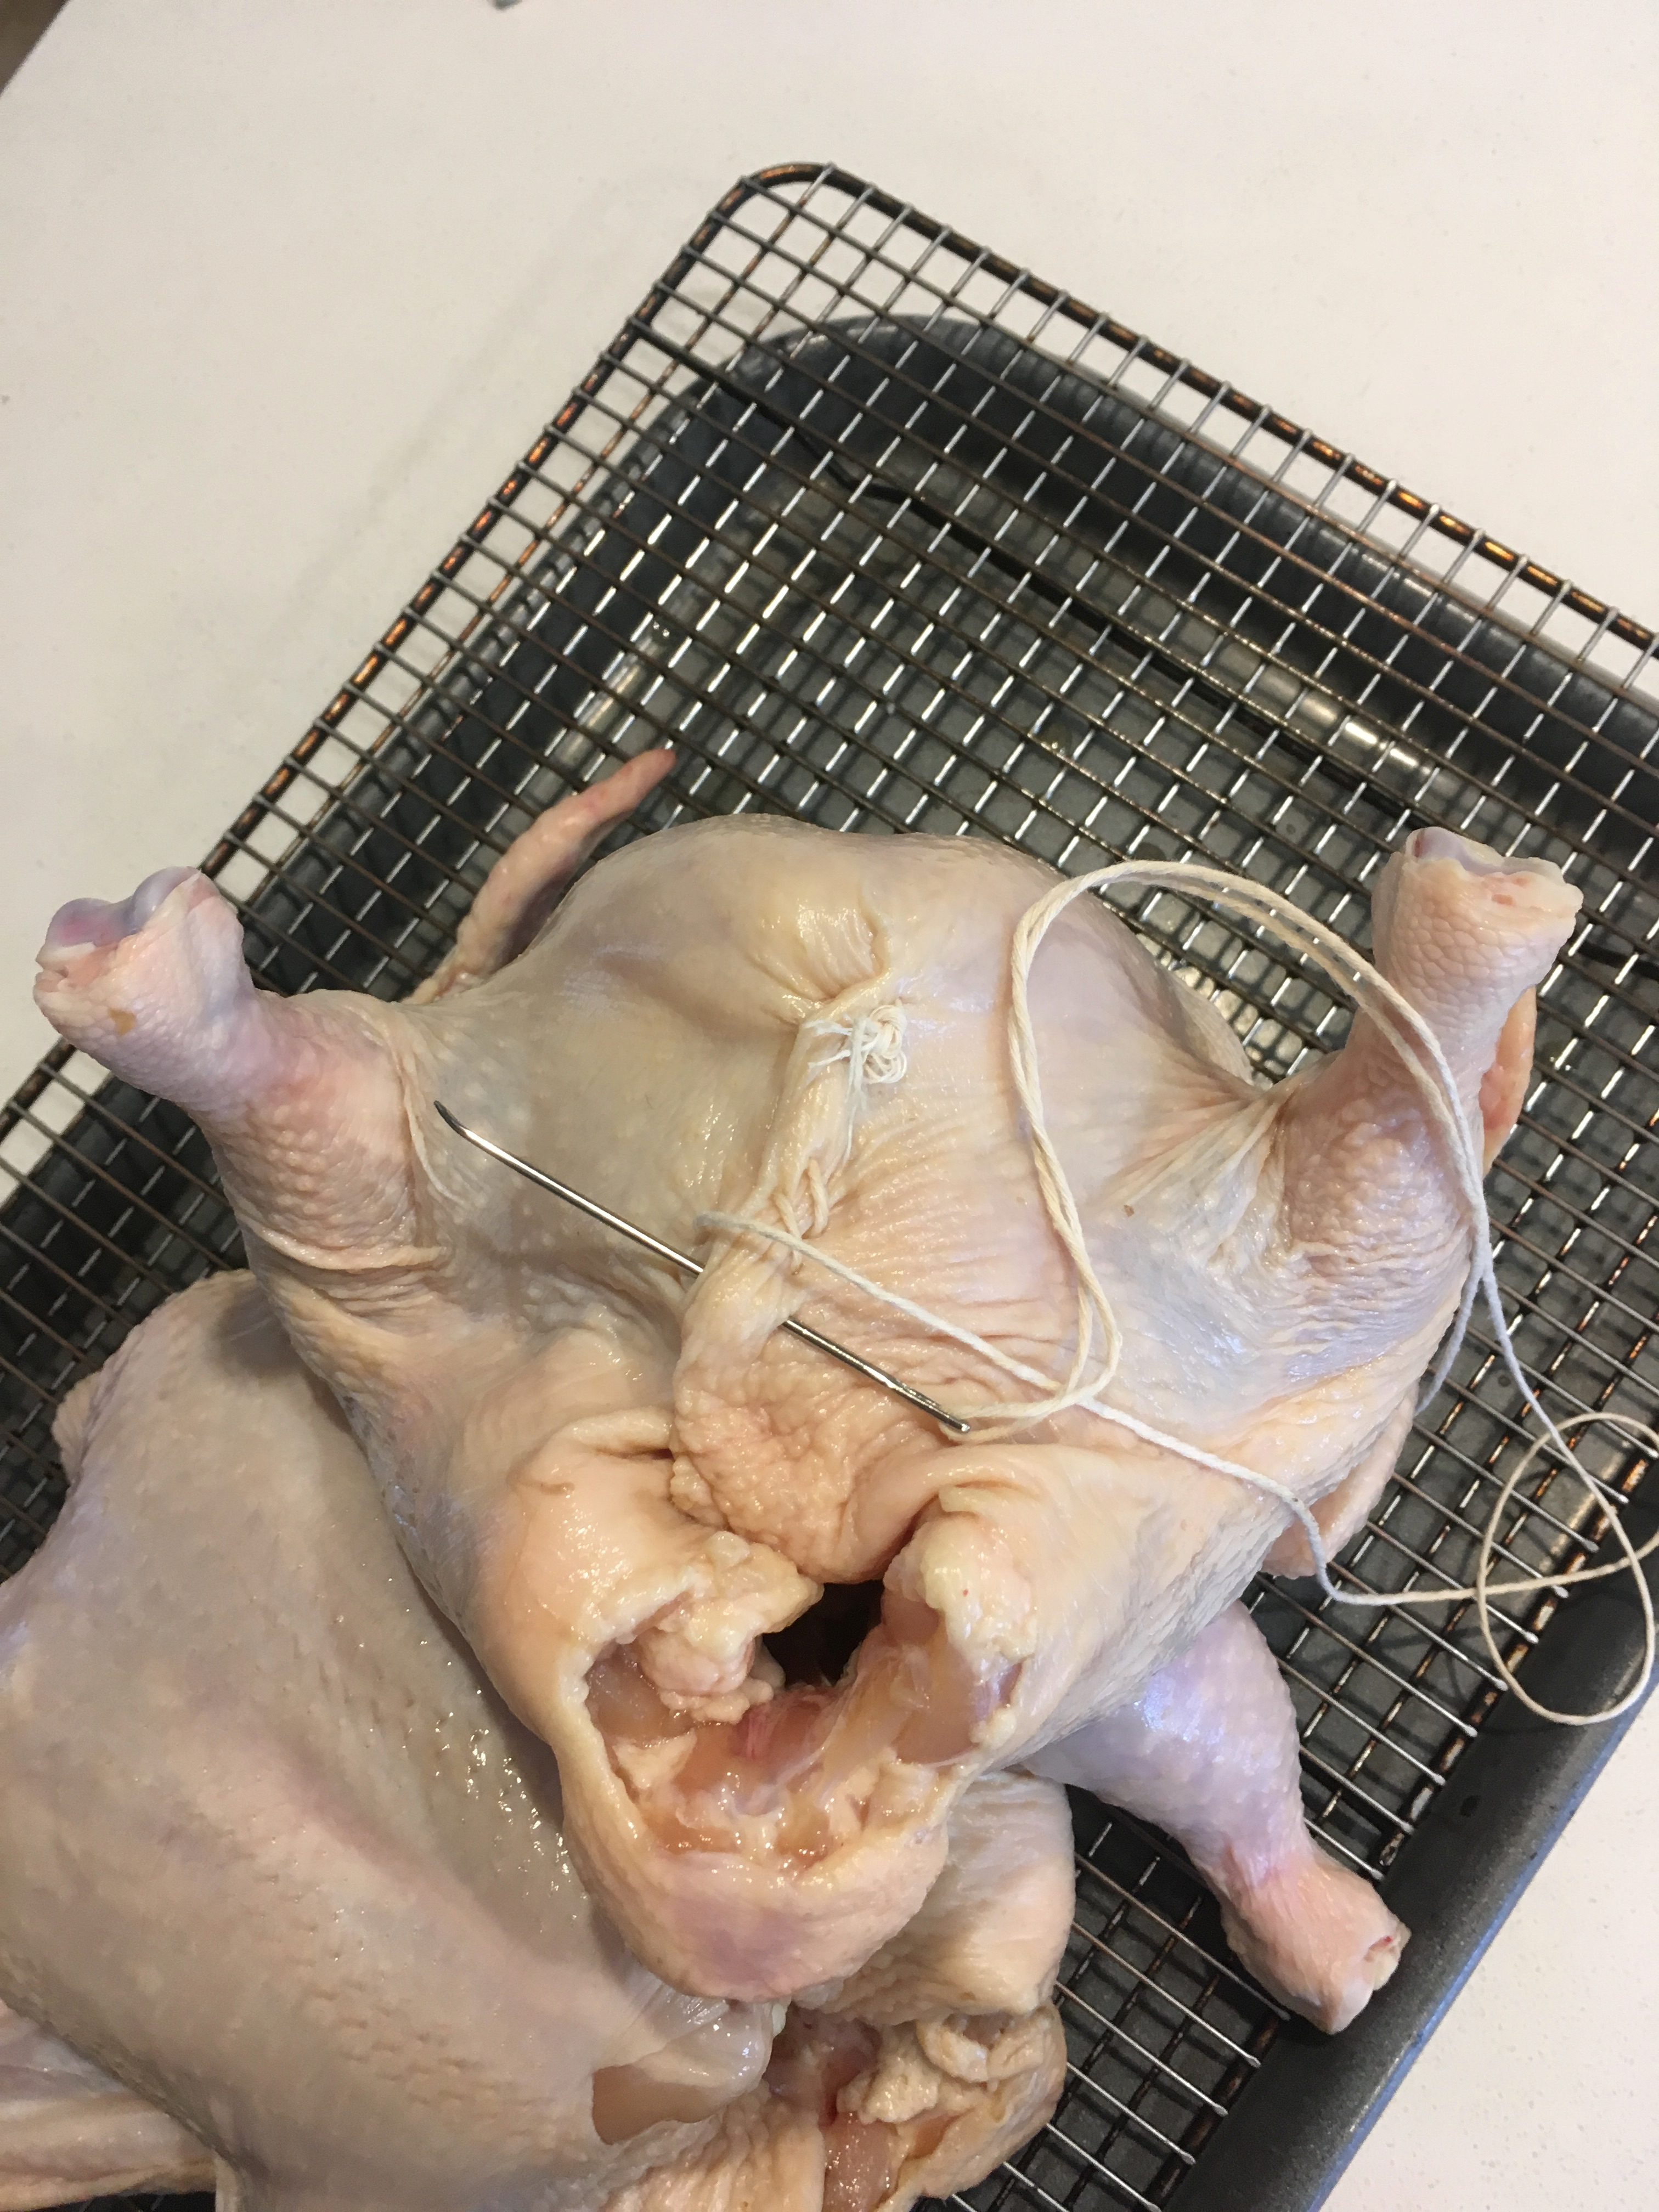
\includegraphics[width=0.25\textwidth]{\imageDir/\fileName/IMG_3216.jpg} \\
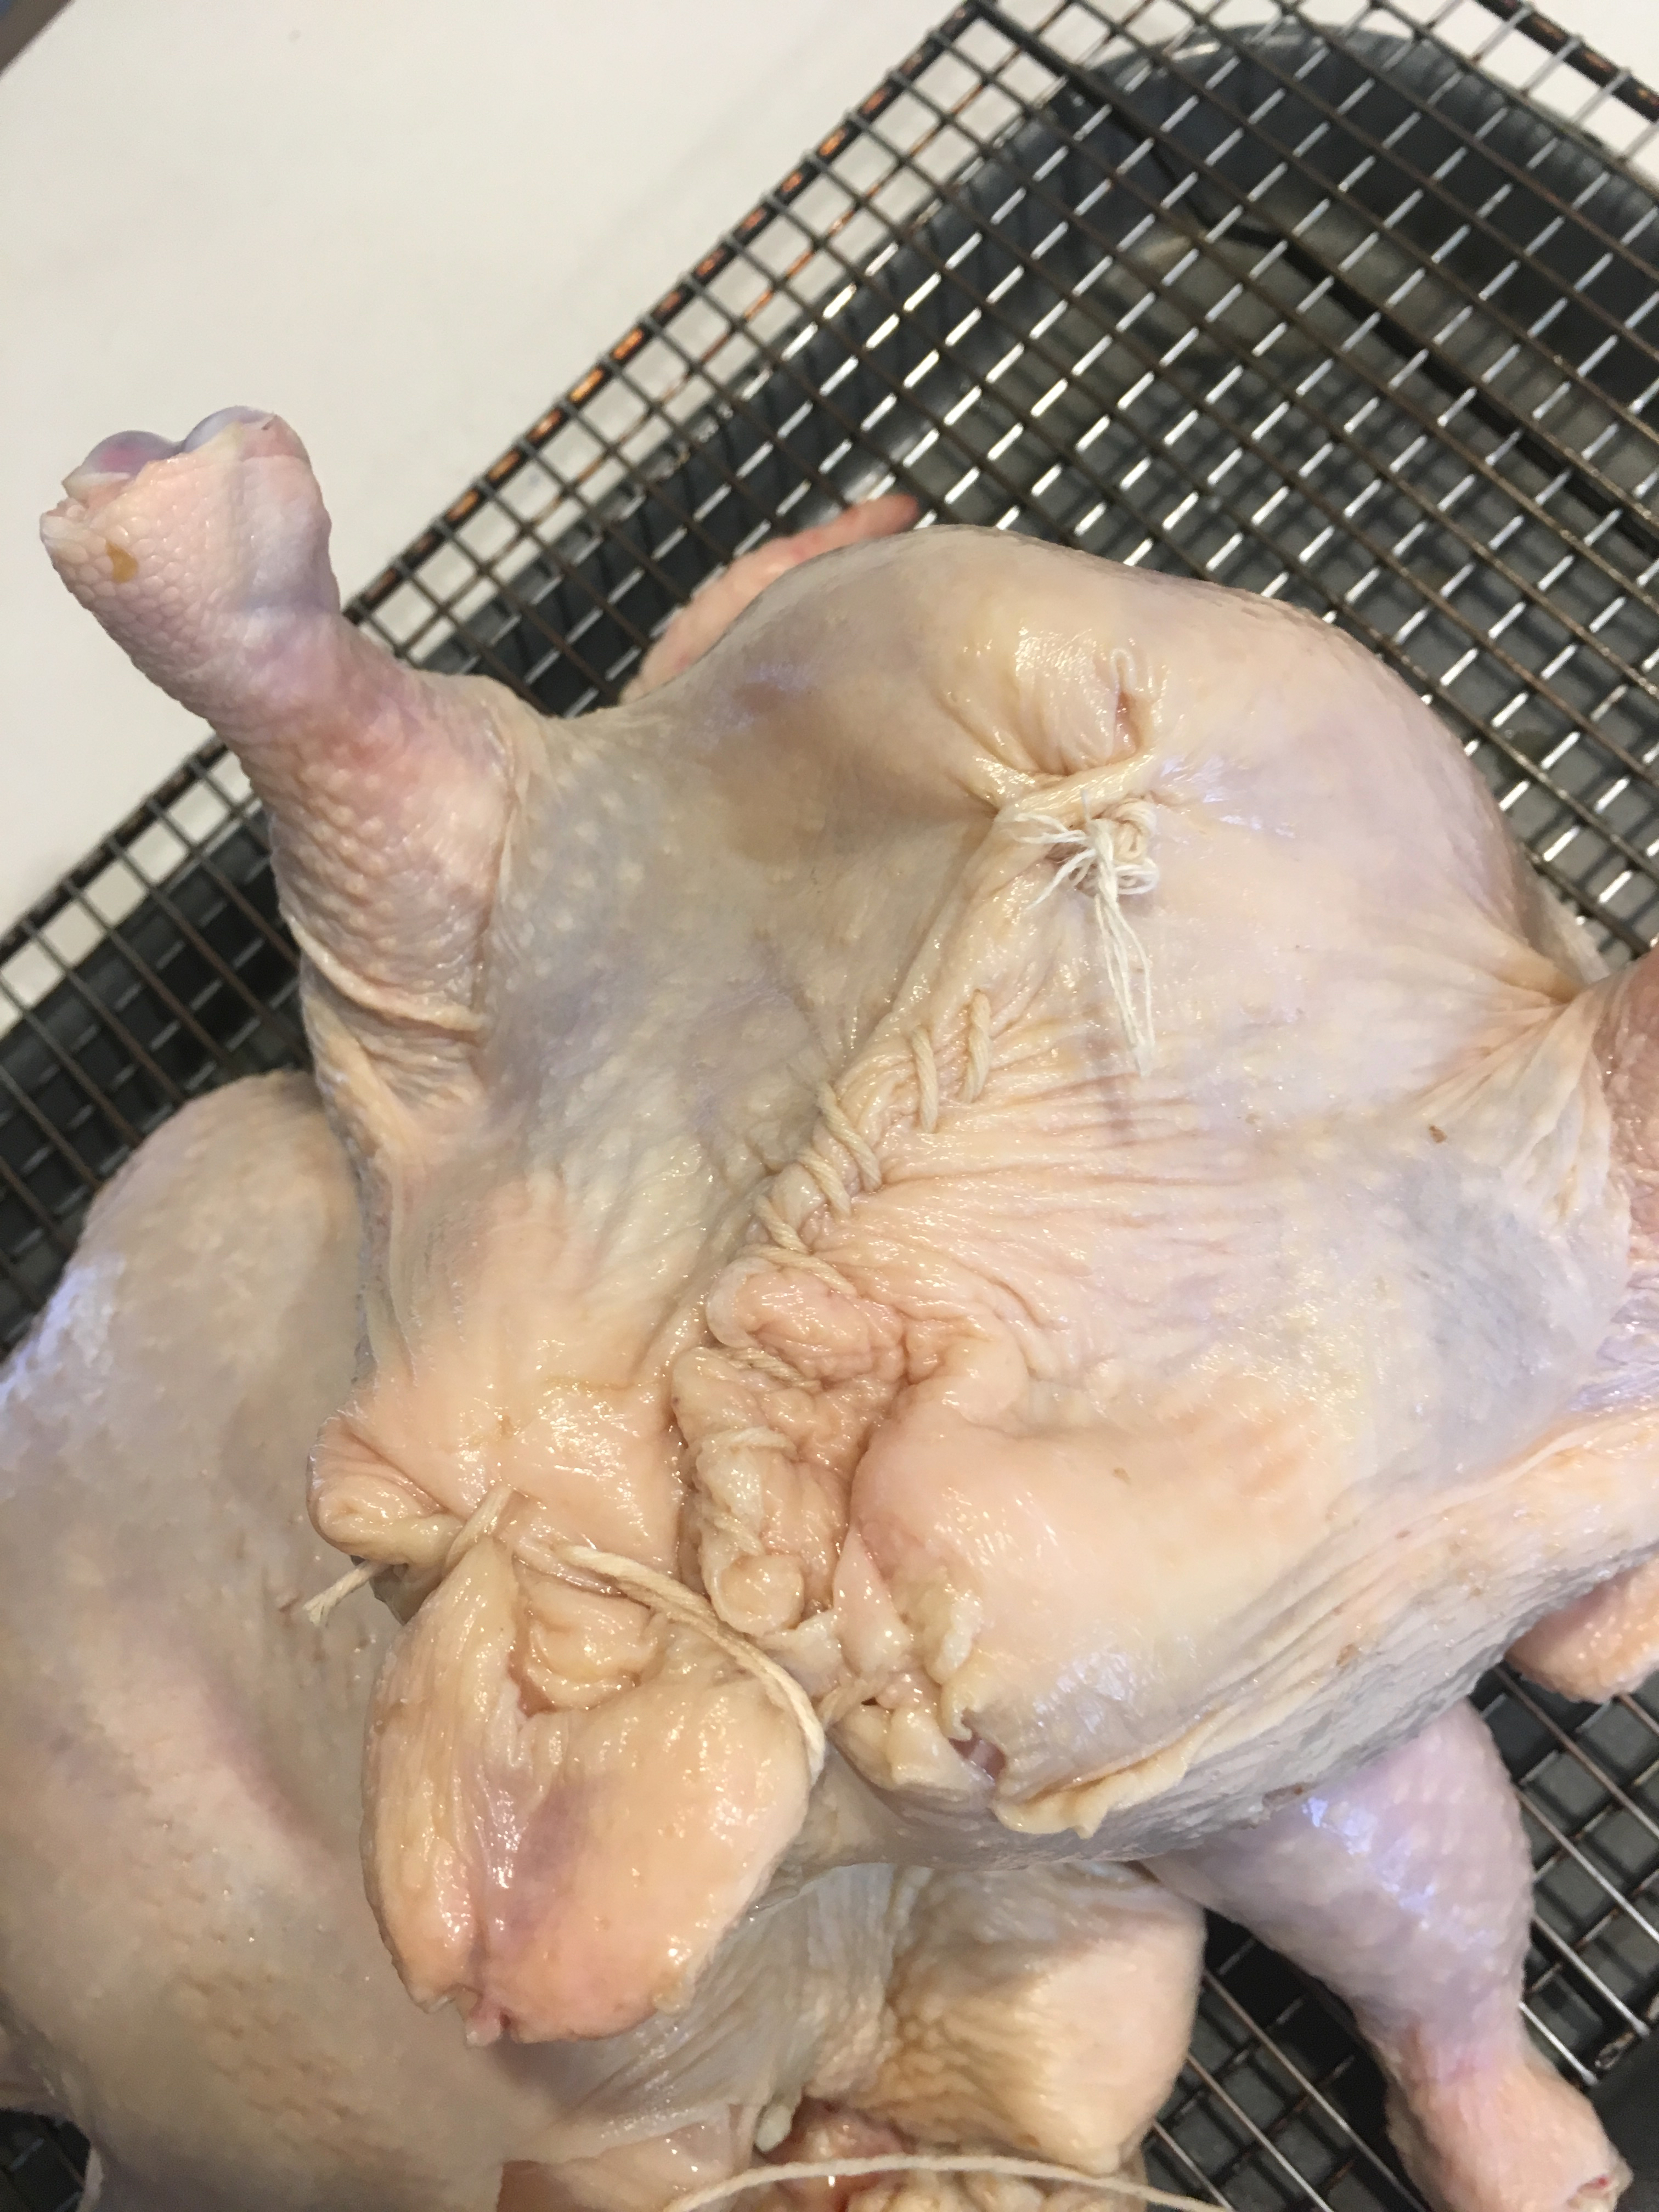
\includegraphics[width=0.25\textwidth]{\imageDir/\fileName/IMG_3217.jpg} &
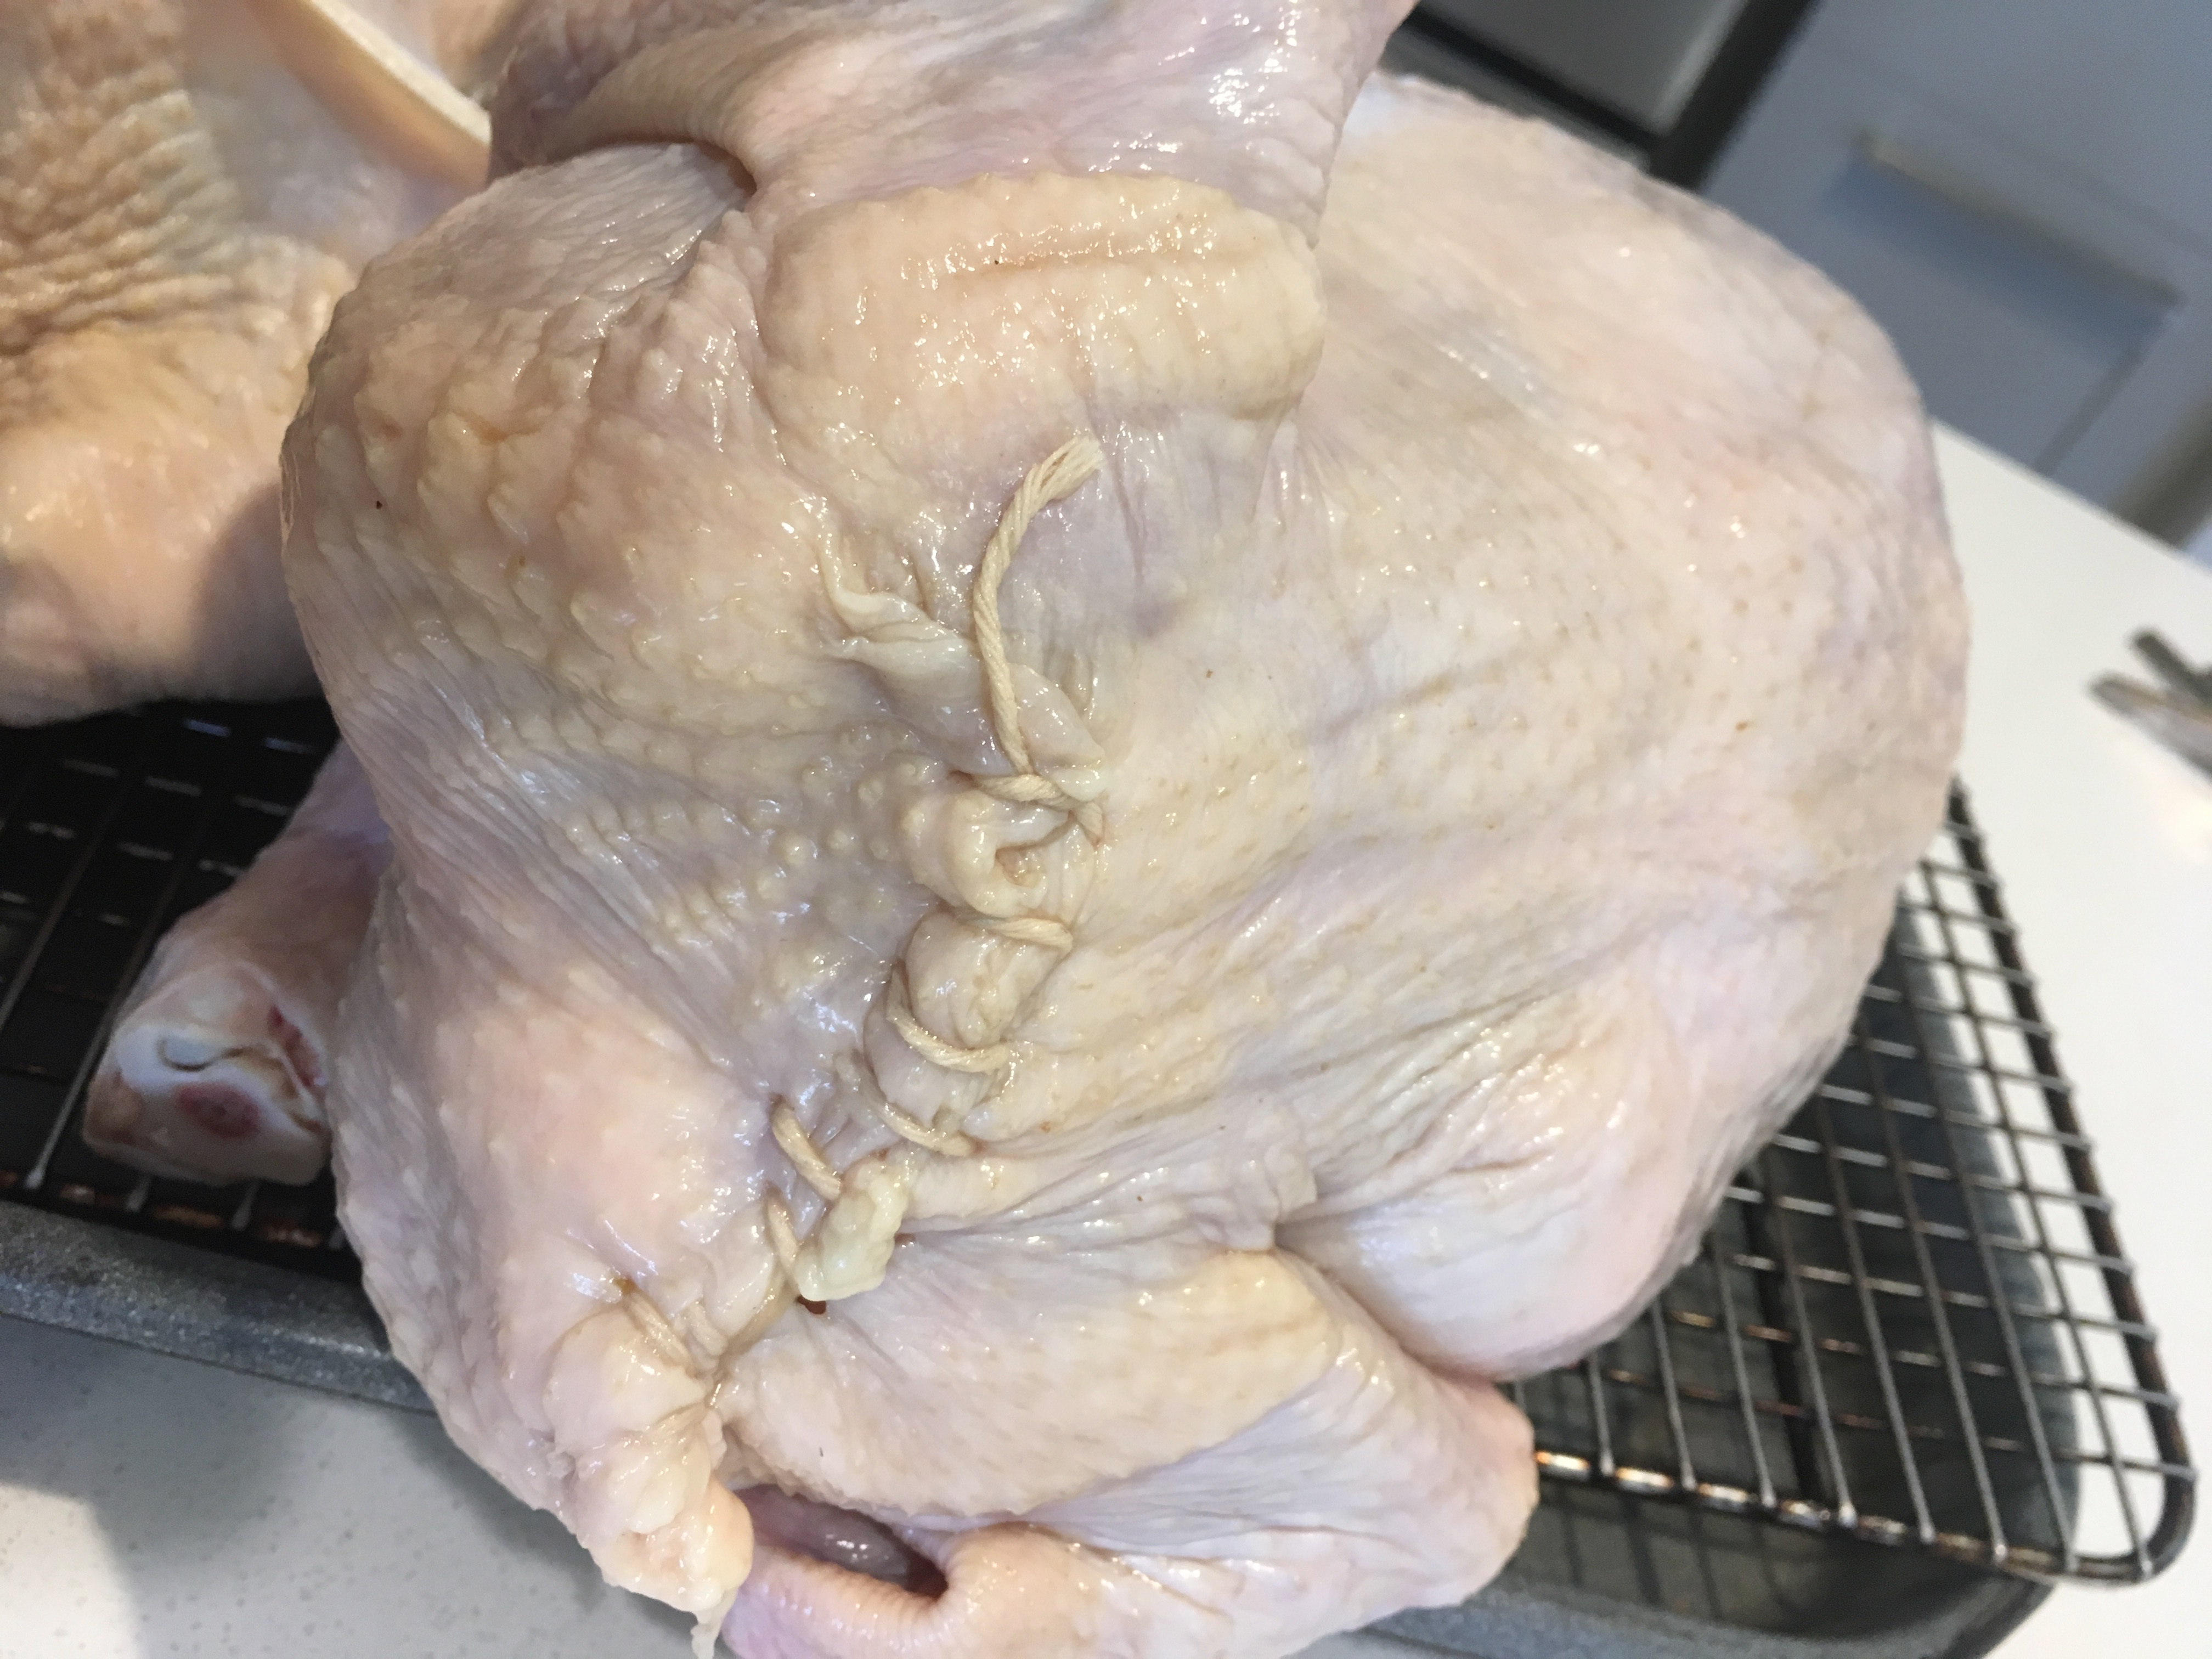
\includegraphics[width=0.25\textwidth]{\imageDir/\fileName/IMG_3218.jpg} &
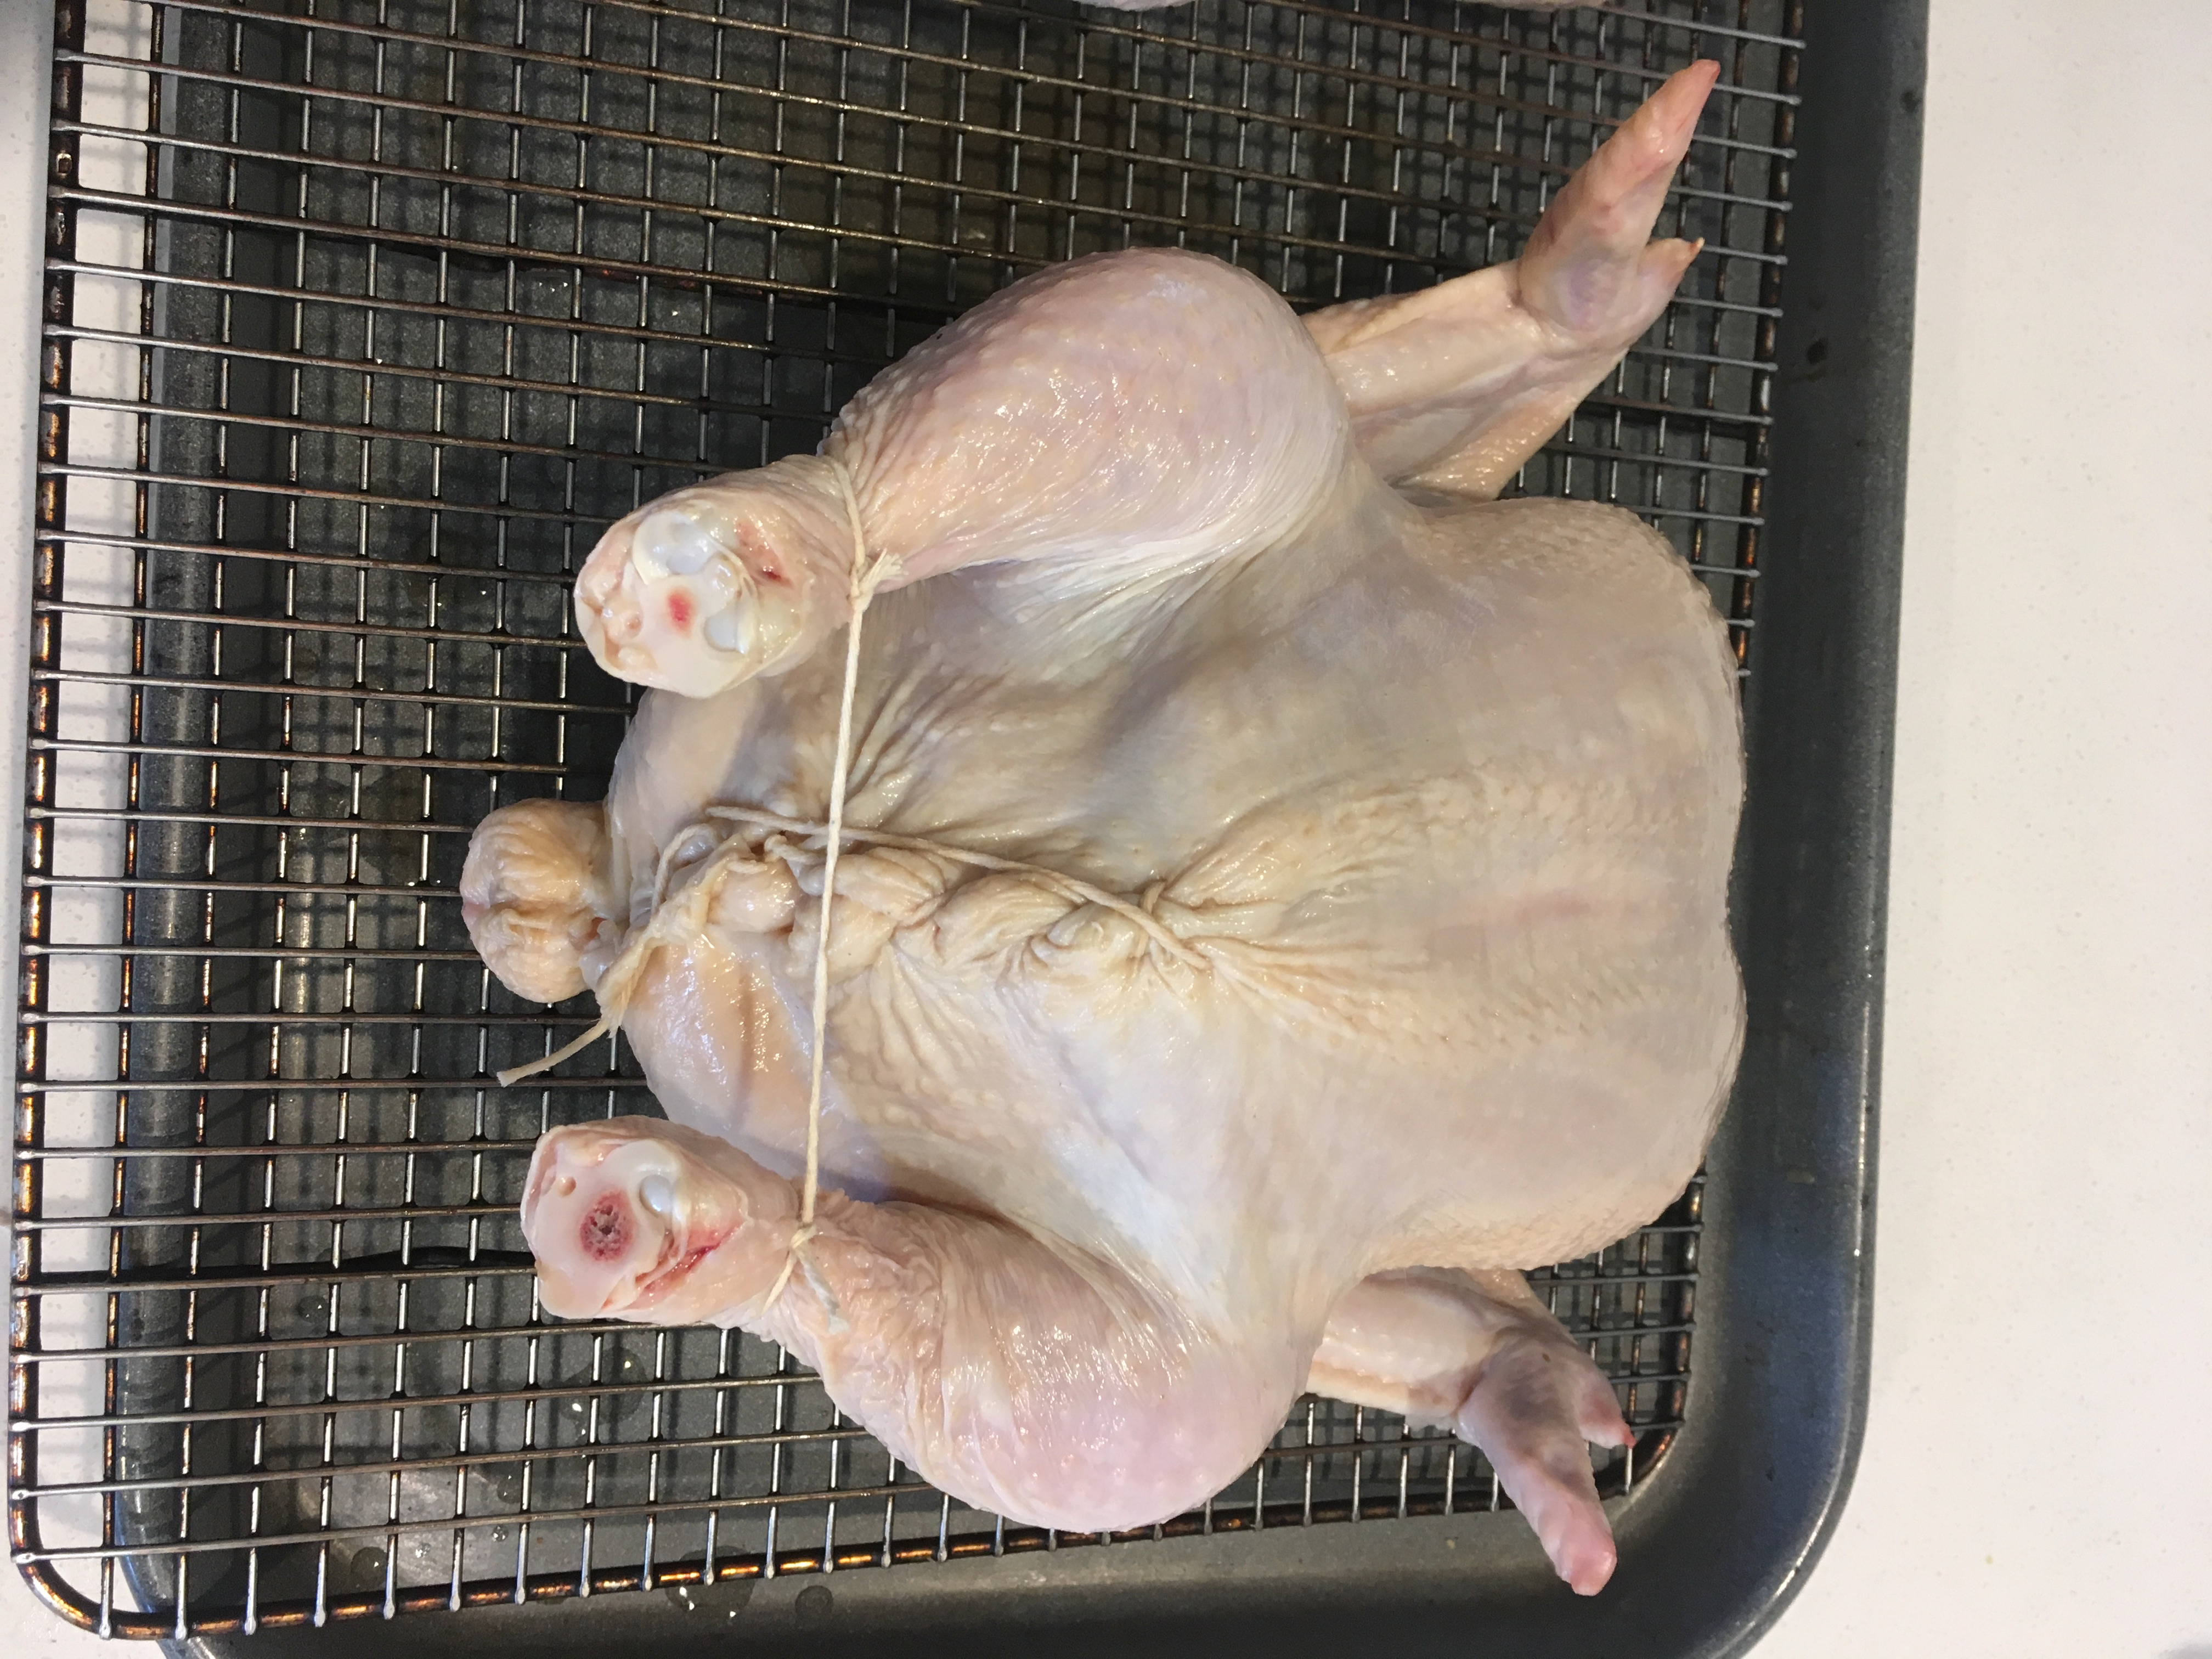
\includegraphics[width=0.25\textwidth]{\imageDir/\fileName/IMG_3219.jpg} \\
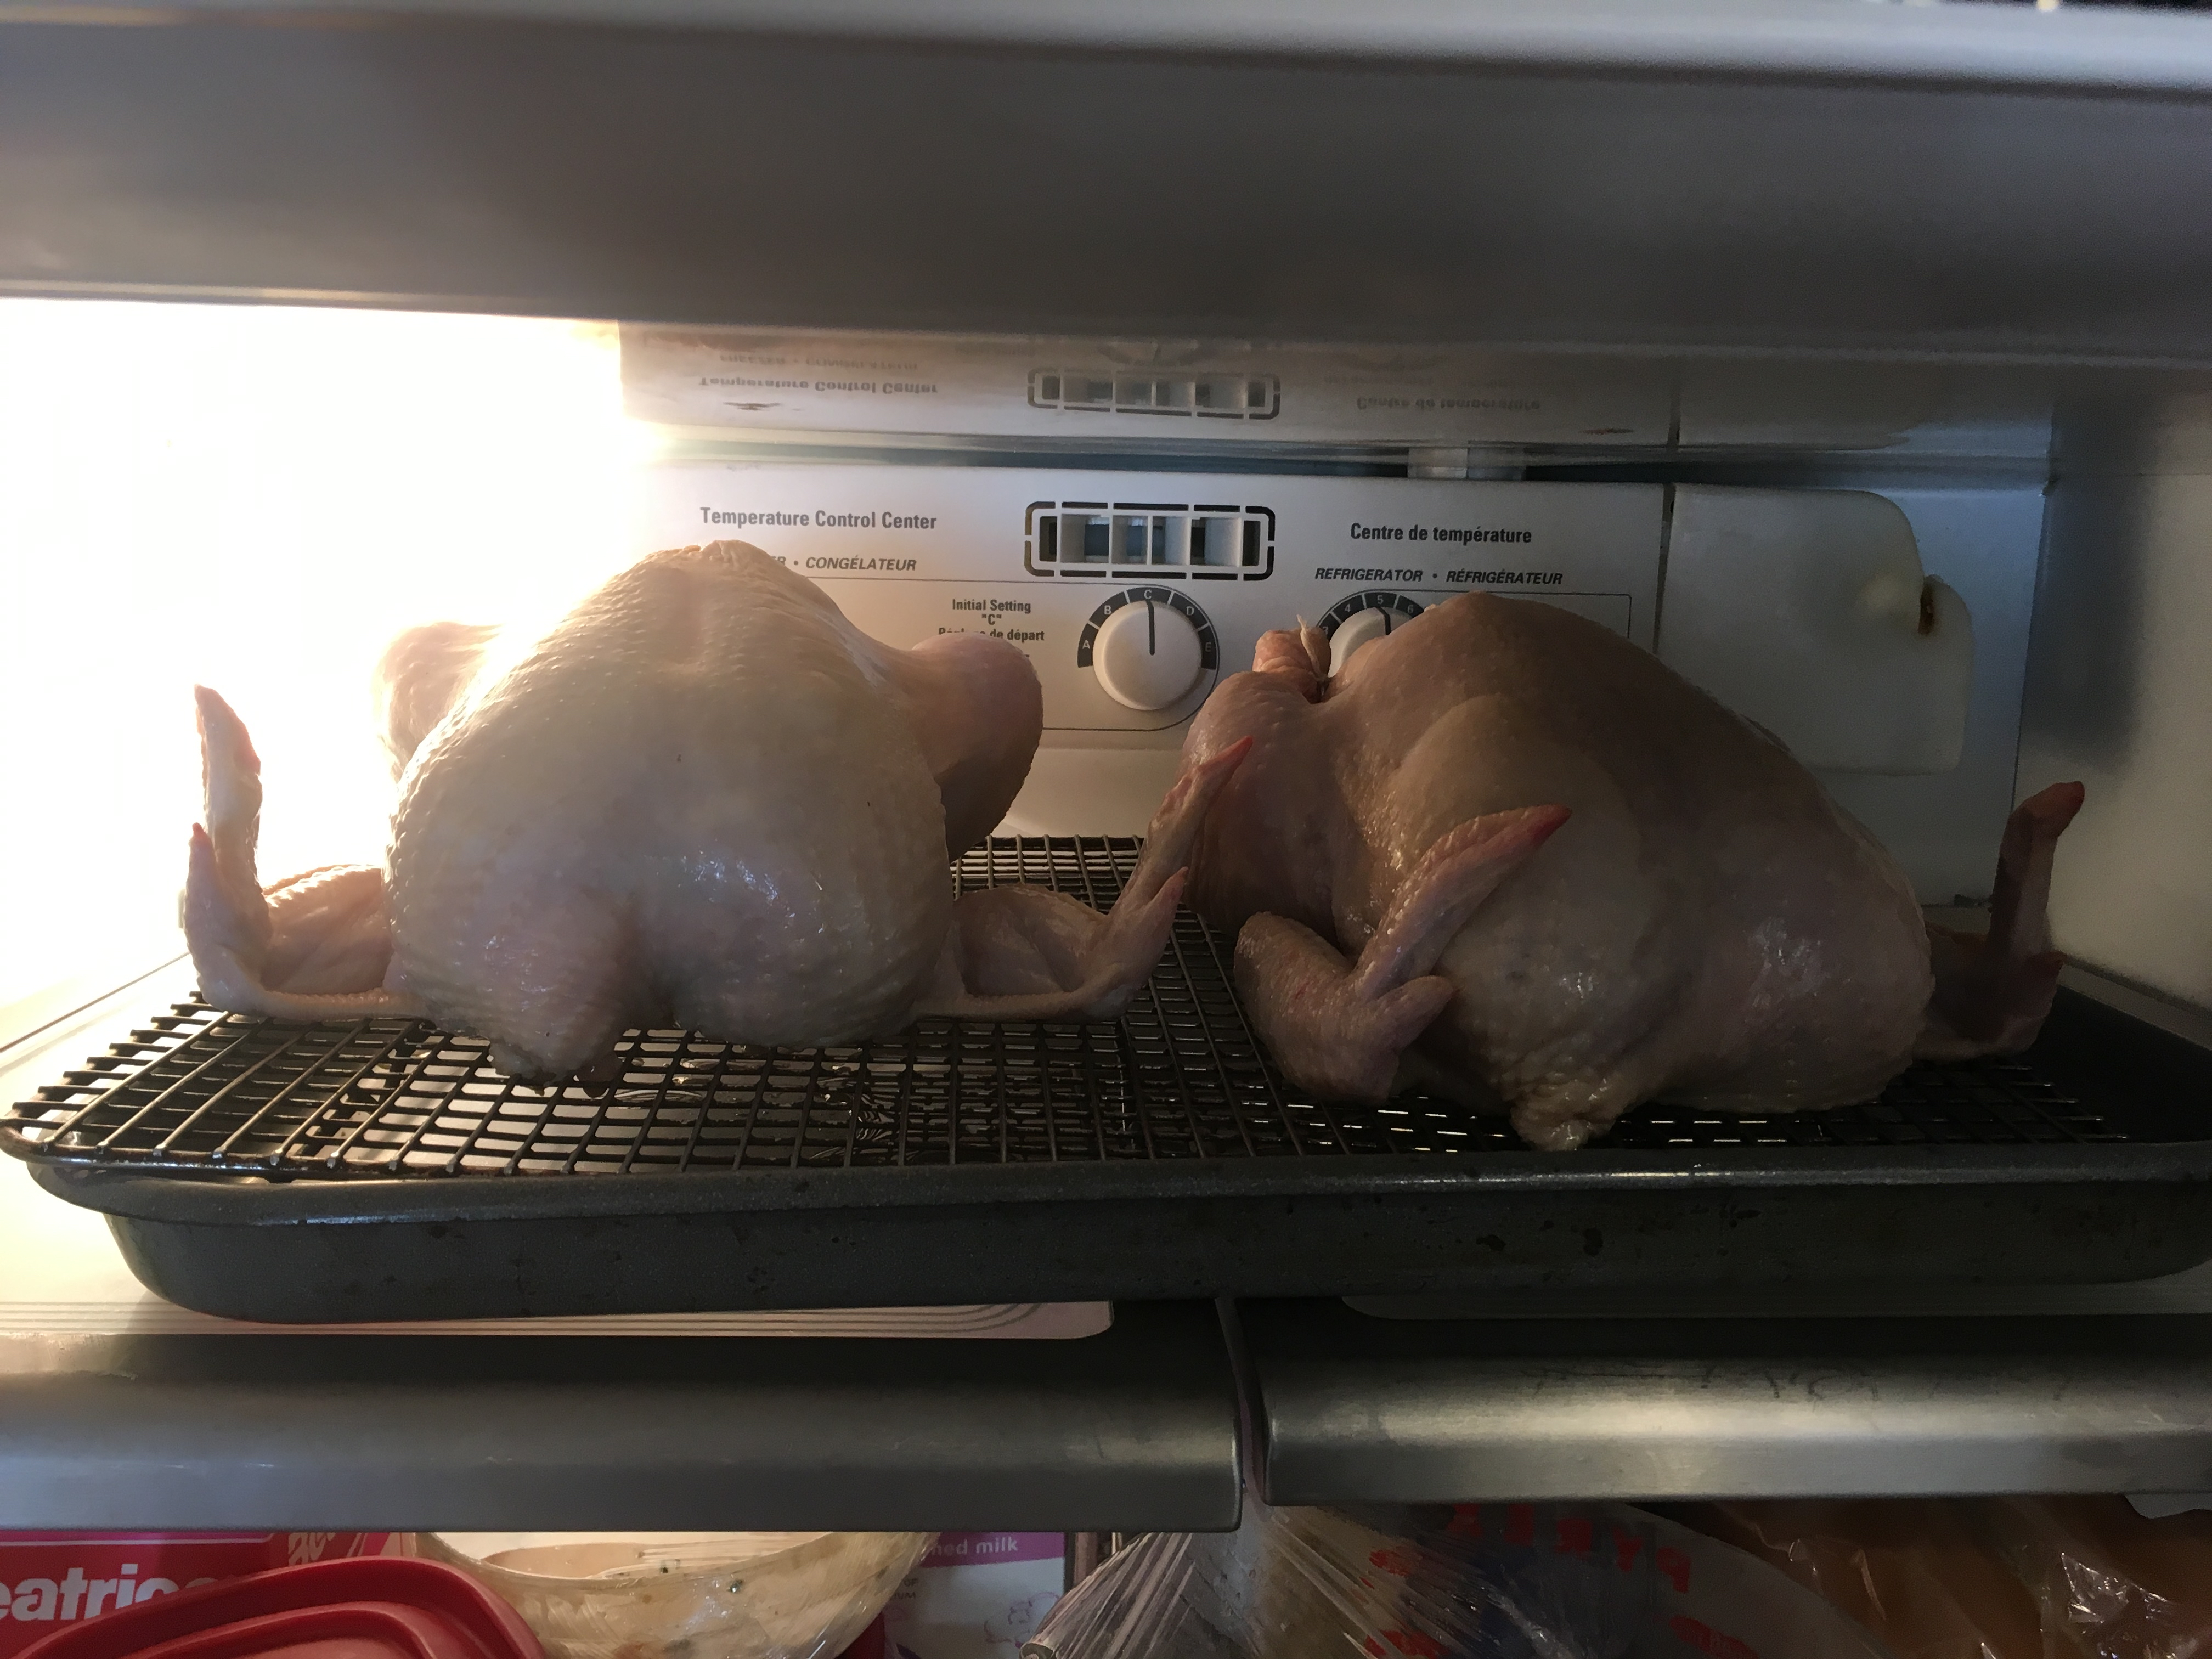
\includegraphics[width=0.25\textwidth]{\imageDir/\fileName/IMG_3220.jpg} &
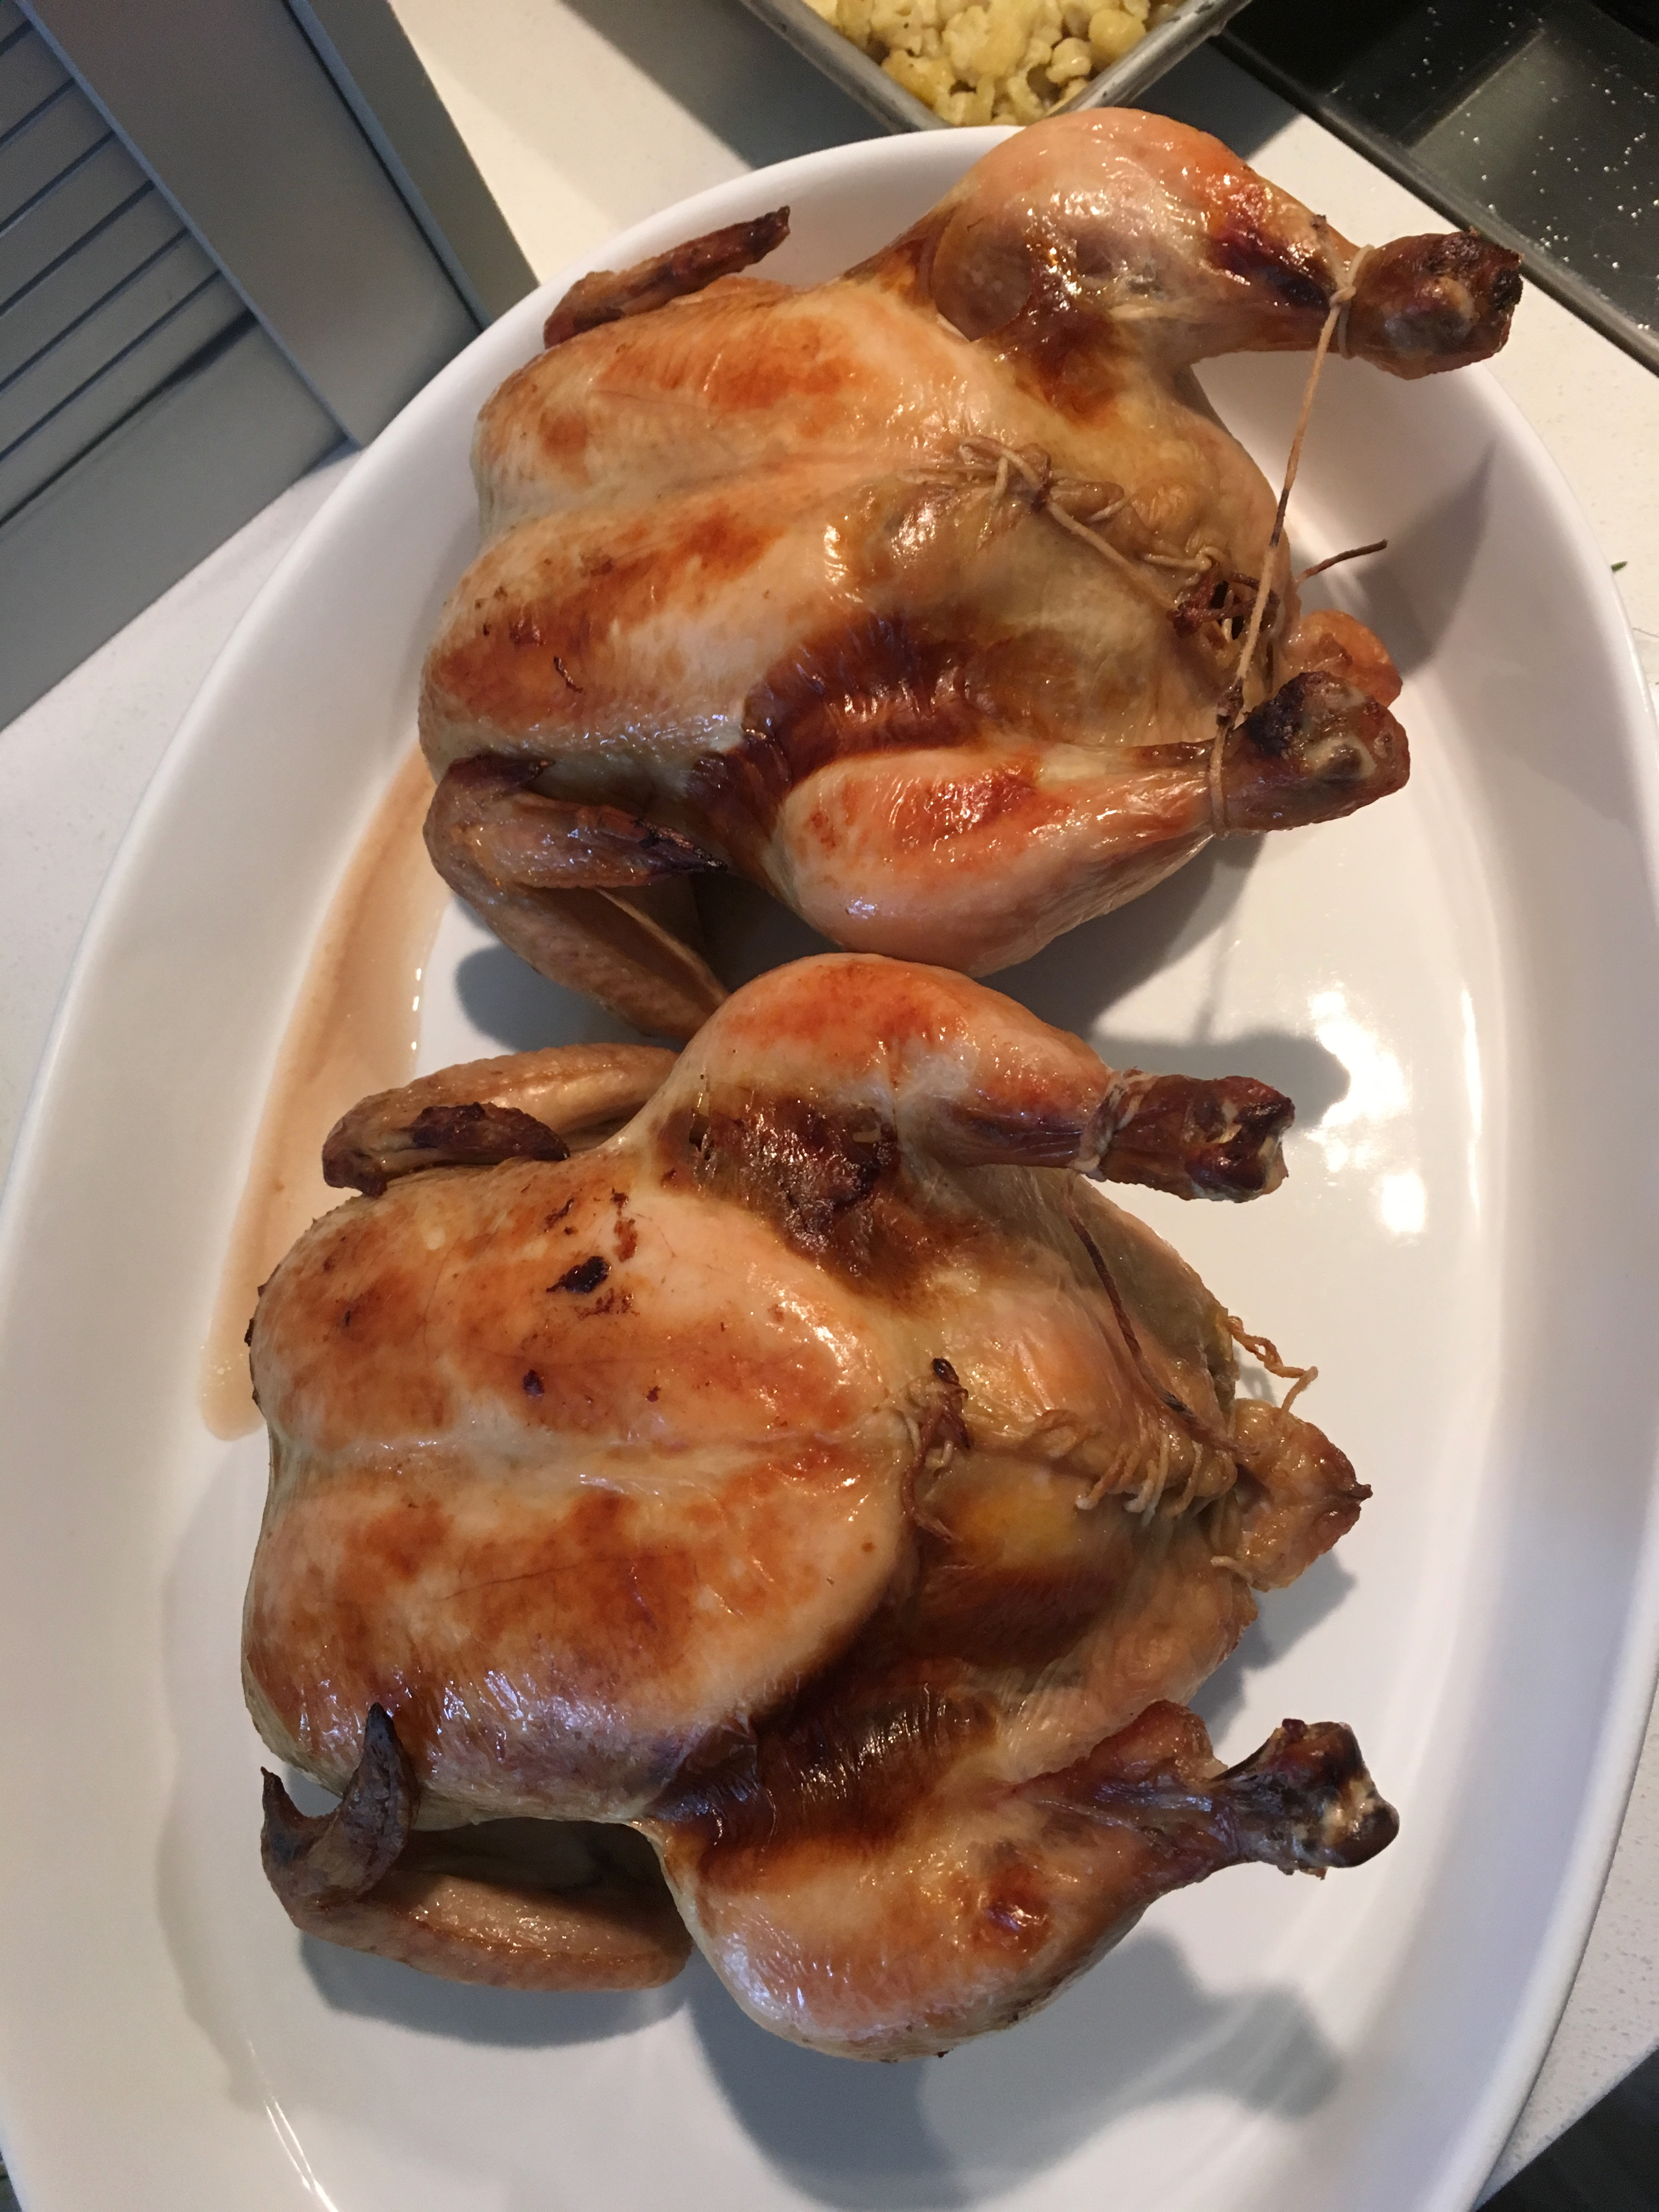
\includegraphics[width=0.25\textwidth]{\imageDir/\fileName/IMG_3228.jpg} \\
\end{tabular}
\end{table}

\end{document}
